\declarecommand{\callout}[1]{\vspace{10pt}\noindent\fbox{\fbox{\parbox{3.1in}{{#1}}}}\vspace{10pt}}

\declarecommand{\projecturl}{\url{http://oscar.cs.stonybrook.edu/api-compat-study}}
\declarecommand{\compatmetric}{weighted completeness}
\declarecommand{\Compatmetric}{Weighted completeness}
\declarecommand{\CompatMetric}{Weighted Completeness}
\declarecommand{\usagemetric}{API importance}
\declarecommand{\Usagemetric}{API importance}
\declarecommand{\UsageMetric}{API Importance}
\declarecommand{\unwusagemetric}{unweighted API importance}
\declarecommand{\Unwusagemetric}{Unweighted API importance}
\declarecommand{\UnwusageMetric}{Unweighted API Importance}
%\declarecommand{\byinst}{{\tt by-inst}}
%\declarecommand{\byvote}{{\tt by-vote}}
\declarecommand{\osversion}{Ubuntu Linux 15.04}
\declarecommand{\osdist}{Ubuntu/Debian Linux}
\declarecommand{\osarch}{x86-64}
\declarecommand{\kernelversion}{3.19}
\declarecommand{\osinstaller}{{\tt APT}}
\declarecommand{\packagenum}{30,976}
\declarecommand{\binarynum}{66,275}
\declarecommand{\execnum}{34,376}
\declarecommand{\librarynum}{31,899}
\declarecommand{\syscallnum}{320}
\declarecommand{\popsamples}{2,935,744}
%% dp: The weird typesetting for libc seems excessive
\declarecommand{\libc}{libc}
\declarecommand{\Libc}{Libc}
\declarecommand{\libpthread}{libpthread}
\declarecommand{\glibc}{GNU libc}

\chapter{Revisiting Compatibility Requirements with More Practical Measurement}
\label{chap:syspop}

When implementing the system APIs and abstractions,
system developers routinely make design choice based on
what they believe to be the important and unimportant features of the system.
%Systems engineers and researchers routinely make design choices based on 
%what they believe to be the common and uncommon behaviors of a system.
%For instance, one recent project optimized the {\tt stat} and {\tt open} system calls
%at the expense of {\tt rename} and {\tt chmod}~\citep{tsai15dcache}.
%In the case of a general-purpose OS, determining
%exactly what the common case is can be challenging.
However, a developer's view of what APIs are important
may be skewed heavily towards that developer's preferred workloads.
%the choice of what features matter skews heavily towards
%workloads particular developers use.
Similarly, developers struggle to evaluate the impact of a 
change that affects backward-compatibility,
primarily because of a lack of metrics.
Deprecating an API is often a lengthy process, wherein
users are repeatedly warned 
and eventually some applications may still be broken.
%For example, a range of security problems arise from the ill-specified behavior of the {\tt signal} system call~\citep{zalewski01signals,cert-signals}.
%Despite 15 years of warnings to move to the more secure {\tt sigaction} call,
%{\tt signal} has not been removed from 32-bit x86 Linux,
%% (it was simply not added to x86\_64),
%because many legacy applications use {\tt signal}.
Eliminating or replacing needless, problematic APIs 
can be good for security, efficiency, and maintainability of OSes,
but in practice this is difficult for OS developers to do without tools to analyze API usage.

Many experimental operating systems add a rough Unix or Linux compatibility 
layer to increase the number of supported applications~\citep{zeldovich+histar, aviram10determinator, xax, appavoo2003providing}.
Such systems generally support a fraction of Linux system calls,
often just enough 
to run a few target workloads.
One metric for compatibility or completeness of a new feature
is the count of supported system APIs~\citep{tsai14graphene, TxOS, baumann13bascule, bergan10dos}.
%Unless all system APIs are used equally,
System call counts do not accurately
estimate the fraction of applications or users that could plausibly use the system.
OS researchers would benefit from
the ability to translate
a set of supported system calls 
to the fraction of applications that
can be directly supported without recompilation.  Similarly, it is useful 
to know which additional APIs would enable the largest range of additional applications to run on the system.
%OS maintainers can use such a metric to focus efforts to deprecate or extend an existing API.
%Finally, users may }
In order to indicate general usefulness, a 
good compatibility metric should factor in 
the fraction of users whose choice of applications can be
completely supported on a system.
%A useful compatibility metric should further 
%identify 
%supported applications
%into
%\rev{rewrite}{An even more critical question is
%whether developers can further deduce the fraction of Linux users %that could realistically
%use the experimental system.}
%As we show, this metric
%can both over- and under-approximate the degree to which a prototype
%can meet the needs of real users.

%Simply counting supported system calls or APIs is a very rough number, and researchers need 
%a better metric to evaluate the degree to which their prototype is applicable to real users.

At the root of these problems is a lack of data sets and analysis of
how system APIs are used in practice.
System APIs are simply not equally important: 
some APIs are used by popular libraries and, thus, by essentially every application.
Other APIs may be used only by applications that are rarely installed.
Evaluating compatibility is fundamentally a measurement problem.
%System call counts do not capture this nuance.
%supporting a system call that is commonly used in popular applications
%is more valuable than
%supporting one that is not used at all.
%Users only care whether their software installations will be broken if they adopt a new system prototype.
%System 
%The gap between the count of system APIs
%implemented by a prototype and the fraction of applications and users
%that could adopt the prototype is
%the primary reason that makes the former an unusable metric.  

%This paper bridges the gap between 
%data that is easy for system builders to measure and the 
%metrics they need, contributing 
%%existing metric and the one we actually need, with
% a methodology and thorough study of API usage in \osarch{} \osdist{}.
%Our study statically analyzes all executable and shared library binaries from all
%\packagenum{} packages in the \osdist{} repository, in order
%to identify the system API ``footprint'' of each binary.
%%\rev{emphasize this}{including both executables and shared libraries}.
%%Our analysis only requires application binaries.
%%all the system calls each application can issue (the system call ``footprint'').
%This paper combines the footprint data with data about how frequently 
%each package is installed, which is measured from the Ubuntu and Debian ``popularity contest'' survey data~\citep{ubuntu-popularity, debian-popularity}.
%By combining these data sources, the paper contributes metrics
%which weigh the usage of each system API by estimated usage in real-world installations.


%We will release the data set and analysis tools with this paper.


%% dp: This is pretty repetitive with the text above.  I propose putting it lower in the interest of brevity
%%% \begin{revs}{List who will care}
%%% The following are some examples in which either OS developers or users will
%%% benefit from the data sets and metrics described by this paper:
%%% \begin{compactitem}
%%% \item Maintainers who have to wait for a decade before confirming that an API is close to retirement.
%%% \item Users who need to evaluate the thoroughness of system compatibility before adopting a new OS prototype.
%%% \item Developers who have to assess the impact of an important design decision about system APIs.
%%% \end{compactitem}
%%% \end{revs}

%This paper contributes a data set and analysis tool
%that can answer several practical questions for systems researchers.
%For instance: in a given prototype, which missing APIs would increase the range of supported applications?
%Or, if a given system API is optimized, what widely-used applications
%would likely benefit?  We expect that the ability to match evaluation workloads to modified or supported system APIs
%will be particularly useful.  
%Similarly, this data and toolset can help 
%OS maintainers evaluate the impact of an API change on applications, and can help users
%evaluate whether a prototype system is suitable for their needs.

%We expect similar benefits for developers, such as automatically generating 
%system call level sandboxes~\citep{seccomp}, finding and reaching out to developers of applications using a deprecated API,
%and optimizing the in-memory layout of standard libraries, such as \libc{}.
%For instance,  out of \syscallnum{} system calls on \osarch{} Linux,
%20 system calls are used by no packages in Ubuntu,
%and an additional 58 are used by applications installed on less than 1\% of surveyed systems.

%\fixmedp{Maybe pontificate more about why compat. as a binary property isn't good enough}

%The contributions of this work are as follows:
%\begin{compactitem}
%\item An approach to measuring platform compatibility, suitable for evaluating the relative completeness of prototype systems.
%Rather than considering compatibility a binary property (``will something break?''),
%%yet for prototypes, which are necessarily in-progress,
%we use a fractional metric 
%(``how many programs will not break?'')
%which is better suited to measuring  the progress of 
%a prototype.
%\item A comprehensive data set of current API usage in \osversion{}.  
%\item Analysis and a range of insights into current API usage patterns. For instance, we identify an efficient path to implementing
%a new Linux compatibility layer, maximizing the additional applications per system call.  We also identify
%that usage of many APIs is similarily distributed: some are widely used, and there is a sharp drop with a very long tail
%of rarely or never-used APIs.  As an example, nearly 40\% of libc APIs are used by less than one percent of applications
%on a typical installation. %\fixmedp{check this}
%%, identifying new opportunities for system designers and important considerations for the evaluation of OS prototypes.
%%% meh - this isn't that novel---the data is key
%%\item An efficient static analysis framework can generates API usage profiles from binaries, with high precision and reasonable efficiency.  For instance, our system can analyze the entire Ubuntu repository on a 48-core machine in 2 days.\fixmedp{right?}
%\end{compactitem}
%

% dp: too cutesy?
\section{Some APIs Are More Equal Than Others}
%\section{How to Correctly Evaluate API Compatibility}
\label{sec:syspop:measure}

We started this study from a research perspective, in search of a better way to evaluate
the completeness of system prototypes with a Unix compatibility layer.
In general, compatibility is treated as a binary property
(e.g., bug-for-bug compatibility), which loses 
important information when evaluating a prototype that is almost certainly incomplete.
Papers often appeal to noisy indicators that the prototype probably covers all important use cases,
such as the number of total supported system or library calls, as well as the variety
of supported applications.


These metrics are easy to quantify, but problematic.
Simply put, not all APIs are equally important: some are indispensable (e.g., {\tt read} and {\tt write}),
whereas others are very rarely used (e.g., {\tt preadv} and {\tt delete\_module}).
A simple count of system calls is easily skewed by 
system calls that are variations on a theme (e.g., {\tt setuid}, {\tt seteuid}, and {\tt setresuid}).
Moreover, some system calls, such as {\tt ioctl},
export widely varying operations---some used by 
by {\em all} applications and many that are essentially never used (\S\ref{sec:observation:vector}).
%We use the term {\em vectored system call} for calls, such as {\tt ioctl},
%which essentially export a nested system call table, selected by an opcode argument.
%by {\em any} applications in Ubuntu 
Thus, a system with ``partial support'' for {\tt ioctl}
is just as likely to support all or none of the Linux applications distributed with Ubuntu.



%This paper considers system APIs (``APIs'') broadly:
%this includes system calls, as well as any other means by which OS kernel functionality is
%requested, such as a pseudo-file system ({\tt /proc}).
%This paper also considers
%libraries like libc, which are typically responsible for exporting an API, like POSIX,
%as well as the primary way application developers interact with the OS kernel.
%For applications, system libraries are also system APIs. Modern applications rarely use the kernel interfaces like system calls directly, but instead call library APIs as wrapper or translation layer of kernel interfaces. 
%For Linux platforms, \libc{}, or {\em Standard Library C}, is the most ubiquitously used system libraries, providing a large fraction of
%general-purpose APIs commonly used by every application.


%%%  for the rest of the paper) as channels upon which
%%% applications request system functionalities,
%%% based on the contract between users and OS developers.
%%% The basic form of APIs on UNIX platforms is the system call,
%%% but others exist.
%%% For example, other APIs can be used through accessing system pseudo files or devices,
%%% such as {\tt /proc} files,
%%% or even communicating with administrative services using specific protocols (not covered in this paper).
%%% Although a API can contain multiple channels ---
%%% for instance, {\tt stat} system call provides several file attributes, or a pseudo file can be either read or written ---
%%% we group the usage data by system call numbers, vectored system call operation codes, and file paths,
%%% as the basic granularities of our analysis.  



%and easy to miss important cases in single system calls with a wide variety of options, such as {\tt ioctl}.

One of the ways to understand the importance of a given interface
is to measure its impact on end-users.  
In other words, if a given interface were not supported, how many users would notice its absence?
Or, if a prototype added a given interface, how many more users would be able to use the system?
%% probably don't need this note to Bianca
%\note{Drop footnote here.}
%\footnote{This assumes that the prototype is well-supported by the developers, and the maintainers have reasonable
%  installation instructions, are responsive to bug reports, etc.  The issues around maturity and support
%  of research prototypes are orthogonal to the question of which APIs need to be present
%  in a proof-of-concept system.}
To answer these questions, we must consider both the 
difference in API usage
among applications,
and the popularity of applications among end-users.
We measure the former by analyzing application binaries,
and determine the latter from installation statistics collected
by Debian and Ubuntu~\citep{ubuntu-popularity,debian-popularity}.
An {\bf installation} is a single system installation, and can 
be a physical machine, a virtual machine, a partition in a multi-boot system,
or a chroot environment created by {\tt debootstrap}.
Our data is drawn from over 2.9 million installations
(2,745,304 Ubuntu and 187,795 Debian).
%\fixmedp{Add a summary about how big this data set is (i.e., millions of systems)}
%Although difficult to measure directly, we approximate this based on package installation statistics~\citep{ubuntu-popularity}.


%%% This paper borrows the notion of installations from the package installation statistics.
%%% An {\em installation} represents a set of software installed in a standalone environment
%%% using the provided Ubuntu or Debian package installer.
%%% An installation does not necessarily represent a physical machine;
%%% it can be a partition in a multi-boot system,
%%% a virtual machine,
%%% or even a subsystem installed by 

We introduce two new metrics: one for each API, and one for a whole system.
For each API, we measure how disruptive its absence
would be to applications and end users---a metric we call {\bf  \usagemetric{}}.
For a system, we compute a weighted percentage we call {\bf \compatmetric{}}. 
For simplicity, we define a {\bf system} as a set of implemented or translated APIs,
and assume an 
application will work on a target system if the application's API footprint is implemented on the system.
These metrics can be applied to all system APIs,
or a subset of APIs,
such as system calls 
or standard library functions.
%pseudo-file system interfaces ({\tt /proc}),
%device interfaces ({\tt /dev}), or standard library functions.
%These metrics , and is fully generalizable to other families of OS distributions.



This paper focuses on \osdist{}, as it is a well-managed Linux distribution with a wide array of 
supported software, which also collects
package installation statistics.
The default package installer on \osdist{} is \osinstaller{}.
A {\bf package} is the smallest granularity of installation, typically
matching a common library or application.
A package may include
multiple executables, libraries, and configuration files.
Packages also track dependencies, such as a package containing 
Python scripts depending on the Python interpreter.
%Note that a package may install multiple executables,
%but the granularity of a package
%typically matches a single application or a set of 
%common, supporting libraries.
%one or more application binaries, but installation statistics are only collected
%at package granularity.
\osdist{} installation statistics are collected at package granularity
and collect several types of statistics.
This study is based on
data of how many
Ubuntu or Debian installations
installed a given target package.
%Other installation statistics are ignored,
%because they do not provide complete information about users' actual choices of packages.}
%\byinst{} shows how many systems installed the package,
%and \byvote{} shows how many systems regularly use the package.
%We calculate our measurements based on both data, depending on
%whether one is interested in supporting
%{\it all} packages installed on a system, or prioritizing {\it important} packages.

%%% For a system, a package is the smallest unit of installation.
%%% %by the package installer.
%%% Each package is a set of files that will be placed into the
%%% file systems. %when the package is installed.
%%% Note that a package does not always include standalone executables.
%%% Other files that can be found in a package
%%% includes scripts, shared libraries, configuration files,
%%% or even kernel extensions (modules).
%%% For those packages that do not include executables,
%%% our study tracks their dependencies. %of those packages.
%%% For example, a package containing Python scripts will depend on
%%% the Python package.
%%% We mark both packages as compatible if Python itself is supported.



For each binary in a package---either as a standalone executable or shared 
library---we use static analysis to identify all possible APIs the binary could call,
or the {\bf API footprint}.
The APIs can be called from the binaries directly,
or indirectly through calling functions exported by other shared libraries.
A package's API footprint is the union of the API 
footprints of each of its standalone executables.
We weight the API footprint of each package by its installation frequency
to approximate the overall importance of each API.
%Based on installation statistics of the package, we approximate the transitive importance of the system calls in each binary's footprint.
Although our initial focus was on evaluating research,
our resulting metric and data analysis provide insights for
the larger community, such as trends in API usage.



% Bug-for-bug compatibility beyond our scope; techniques largely orthogonal to this study; we assume that, once a given system call (say write) is supported and works for a reasonable sample of applications, handling edge cases should be straightforward engineering.  That said, for system calls 

%%% Put current metric discussion here

%% Then a subsection on approach and assumptions



\begin{comment}
API compatibility is one of most important system properties, for maintaining the availability of the whole system and decoupling the development of the OS and every applications.
For an OS of the size of Linux or Microsoft Windows, millions of softwares and subsystems are implemented on top of the platform,
counting on the API contracted to provide its services.
If a system engineer decides to change the API,
an inevitable risk is to sweep and update every existing applications accordingly, which are designed and maintained by countless third parties in the world.

Then, why would a system engineer try to change the API of an OS?
The answer is related with the procedure of developing an OS.
When an OS prototype is built, developers have to rely on experiences and instincts to make educated guess about what to be the ideal API of the system.
As time goes by, the OS gains a larger user base, and receives feedbacks about how the API should really be designed.
As soon as a developer realizes that refining the API can effectively improve either efficiency, robustness, security or user-friendliness of the system,
the risk of losing compatibility {\em slightly} can be totally worthy.

Unfortunately, the reality is that system engineers are frighten by the cost of refining the API for being unable to know how compatibility can be effected.
Since there is no data set about the actual usage of the API among applications, they must assume any application developers can potentially depend on the API.
It often takes a very long time, says 6 years \fixmetsai{LSB took 6 years, reference?}, to confirm, announce, communicate or simply wait until the API is officially deprecated.

We argue that knowing the API usage is the first step of understanding and evaluating compatibility.
Instead of using a realistic metric, system engineers often express the affects on API compatibility by numbers of interfaces that are implemented or modified.
Evaluation by counting the interfaces is extremely inaccurate, because every part of the API have different importance among applications.
Some interfaces are simply more frequently used and thus more important than others; for example, the consequence of changing system call {\tt open}, which is used ubiquitously,  is not the same as changing others like {\tt msgget}.
\end{comment}


\begin{comment}
%Bhushan: - Begin here -
Knowing the values of system interfaces among users is the prerequisite of evaluating platform compatibility.
When OS developers test their systems, a common approach is to prepare numerous test cases that exercise individual system interfaces.
It is often a natural thing to do for OS developers to maintain a list of supported system interfaces,
for either development purpose or advertisement.
However, because system interfaces have different values for users, they cannot be equal while evaluating platform compatibility of the OS.
A frequently used system interface should be considered more important for compatibility than a rarely used one.
\end{comment}

\subsection{\UsageMetric{}: A Metric for Individual APIs}

System developers can benefit from an importance metric for APIs,
which can in turn guide optimization efforts, deprecation decisions,
and porting efforts.  
Reflecting the fact that users install and use different software packages,
%Because users install different software on different systems, 
we define
\usagemetric{} as the probability that
an API will be indispensable to 
 at least one application on a randomly selected 
installation.
We want a metric that decreases
as one identifies and removes instances
of a deprecated API,
and a metric that will remain high for an indispensable API, 
even if only one ubiquitous application uses the API.



%, the  of that API will decrease.
%Similarly, an \usagemetric{} near 100 percent indicates an API is indispensable,
%at least for one ubiquitous application.
%The unsupported API with the highest \usagemetric{} creates an upper bound on 
%the system's overall  \compatmetric{}.
%For instance, if a system is missing an API with an \usagemetric{} of 20\%,
%the \compatmetric{} will never be higher than 80\% (but could be significantly lower).


%%% Given a complete list of installed applications in an OS installation,
%%% by examining the API footprint of every application,
%%% we can easily determine whether removing an API is disruptive for such an installation.
%%% %The result is a binary property: whether the API is important to
%%% %the installation or not.
%%% However, it is hard to predict what applications an installation will include.
%%% Thus, we define the metric for API usage as the probability
%%% that that target API
%%% is indispensable for an random installation.

\vspace{0.1in}
{\noindent
\fbox{\begin{minipage}{\linewidth}
\setlength{\parindent}{-0.1in}
\setlength{\leftskip}{0.1in}
\setlength{\rightskip}{0.1in}
 Definition: {\bf \UsageMetric{}.} \\
For a given API, the probability that an installation includes
at least one application requiring the given API.
%at least one broken application
%(whose API footprint covers the target API),
%if the target API was removed.
\end{minipage}}}
\vspace{0.1in}

\noindent Intuitively, if an API is used by no packages or installations,
the \usagemetric{} will be {\em zero}, causing no negative effects if removed.
We assume all packages installed in an OS installation are indispensable.
As long as an API is used by at least one package,
the API is considered {\it important} for the installation.
Appendix \ref{sec:defs:usagemetric} includes a formal definition of \usagemetric{}.
 
%% Besides the metric, the popularity of system interfaces can be important development hints as well.
%% Knowing the most and least valuable system interfaces of an OS,
%% the developers can make better decision on prioritizing the maintenance or retirement of the interfaces.
%% More influences of system interface popularity are discussed in \fixmetsai{later section?}.

%We define the popularity of a system interface by the probability that an installation become unsupported if the interface is removed.
%In other word, the popularity indicates the {\em cost} or {\em penalty} of deprecating an interface.

\begin{comment}
\paragraph{Formal Definition.}
A given system installation ($\mathtt{Inst}$)
is a set of packages installed ($\{\mathtt{pkg}_1, \mathtt{pkg}_2, ..., \mathtt{pkg}_k \in \mathtt{Pkg}_\mathtt{all}\}$).
For each package $\mathtt{pkg}$ in the \osdist{} repository,
our framework generates the API footprint as 
${\mathtt{Footprint}}_\mathtt{pkg} = \{\mathtt{api}_1, \mathtt{api}_2, ..., \mathtt{api}_k \in \mathtt{API}_\mathtt{all}\}$.  
For an API supported by the OS, we calculate the \usagemetric{} as the product 
of probabilities that an installed package will require this API.
This is calculated as follows:
\begin{align*}
&\mathtt{Dependent}_\mathtt{api} = \{\mathtt{pkg}|\mathtt{api} \in \mathtt{Footprint}_\mathtt{pkg}\} \\
&\mathtt{Importance}(\mathtt{api}) = Pr\{\mathtt{Dependent}_\mathtt{api} \bigcap \mathtt{Inst} \neq \emptyset\} \\
&= 1 - Pr\{\forall \mathtt{pkg} \in \mathtt{Dependent}_\mathtt{api}, \mathtt{pkg} \notin \mathtt{Inst}\} \\
&= 1 - \prod_{\mathtt{pkg} \in \mathtt{Dependent}_\mathtt{api}} Pr\{\mathtt{pkg} \notin \mathtt{Inst}\} \\
&= 1 - \prod_{\mathtt{pkg} \in \mathtt{Dependent}_\mathtt{api}} (1 - \frac{\text{installation of $\mathtt{pkg}$}}{\text{total installation}})
\end{align*}
\end{comment}


\subsection{\CompatMetric{}: A System-Wide Metric}

We also measure compatibility at the granularity of an OS,
which we call \compatmetric{}.
\Compatmetric{} is the fraction of applications that are likely to work,
weighted by the likelihood that these applications will be installed on a system.
%\fixmedp{check this synopsis}
% function of the APIs supported, weighted by the popularity 
%of the applications that require these APIs.

The goal of \compatmetric{} is to measure the degree to which a
new OS prototype or translation layer is compatible with a baseline OS.
In this study, the baseline OS is \osdist{}.



%%  as a function of the API footprint of each potentially-installed
%% application, weighted by the popularity of each application.
%% We introduce the metric , which we define in terms of an OS installation (i.e.,
%% the libraries and applications) and a target API implementation, which may provide a subset
%% of the original system's APIs.


%% An accurate metric for API compatibility must take into account at least two factors:
%% \begin{compactenum}
%% \item For each interface in the API, what are the applications that rely on it and could be affected if the interface is removed? ({\em application footprint})
%% \item For each application, how many installations of the system in the world has included it? ({\em application popularity})
%% \end{compactenum}


%% \fixmedp{Term for each call, vs system overall: API Importance and Effective Coverage?}

%% To accurately evaluate compatibility, we design a metric that is quantifiable, \fixmetsai{one more word here}, and easy to interpret.

\begin{comment}
We defined {\bf platform compatibility} as "{\em the probability of porting any installation of an OS distribution onto the target OS without any effort}".
The definition of an {\em installation} is a combination of application setup on a standalone OS instance.
An Installation can exist on physical machines,
or any machines of generalized sense such as a virtual machines, containers or subsystems.
In our model, installations represent customers of the OS, who are considered equal when providing any services.
\end{comment}

\vspace{0.1in}
%\fixmetsai{Find a good name for our metric} 
{\noindent
\fbox{\begin{minipage}{\linewidth}
\setlength{\parindent}{-0.1in}
\setlength{\leftskip}{0.1in}
\setlength{\rightskip}{0.1in}
Definition: {\bf \CompatMetric{}.} \\
For a target system, the fraction of applications supported,
weighted by the popularity of these applications.
%For any installation, the expected fraction of installed applications that can work on the target OS.
%\fixmedp{shouldn't the weight go in the definition?}
%\Compatmetric{} is the total size of all supported applications,
%weighted by the popularity of each application.
\end{minipage}}}
\vspace{0.1in}

%\noindent In terms of porting effort, we are primarily interested in avoiding code changes, 
%such as {\tt \#ifdef LINUX}; although we leave this notion somewhat vague.
%We consider recompilation, relinking, or other mechanical processes acceptable.

%% Our analysis framework scans through all available packages in the \osdist{} repository and generates system interface footprint data for individual package.
%% The footprint data is based on static analysis,
%% and it lists all potentially used system interfaces regardless of the applications' runtime coverage. 
%% To build the metric, we also import the package popularity statistics from the official \osdist{} reports~\citep{ubuntu-popularity, debian-popularity}.

The methodology for measuring the \compatmetric{} of a target system's API subset is summarized as follows:
\begin{compactenum}
\item Start with a list of supported APIs of the target system, either identified from the system's source, or as provided by the developers of the system.
\item Based on the API footprints of packages, the framework generates a list of supported and unsupported packages.
\item The framework then considers the dependencies of packages. If a supported package depends on an unsupported package, both packages are marked as unsupported.
\item Finally, the framework weighs the list of supported packages based on package installation statistics.
As with \usagemetric{}, we measure the effected package that is most installed;
\compatmetric{} instead calculates the expected fraction of packages in a typical installation that will work on the target system.
%Specifically, each package's weight is based on 
%and the framework calculates the expected fraction of packages from a typical installation that will work on the target system.
\end{compactenum}
%\fixmedp{``typical installation'' raised some hackles.  Can we either use a different term, or talk more about this concept?}

\begin{comment}
\paragraph{Formal Definition.}
Suppose an OS supports a set of APIs ($\mathtt{API}_\mathtt{Supported}$),
% = \{i_1, i_2, ..., i_n\}$
which is a subset of the APIs of the original system ($\mathtt{API}_\mathtt{all}$).
In this study, $\mathtt{API}_\mathtt{all}$ is the sum of Linux APIs, including
the system call table, sysctl, proc, and so forth.
%(total APIs are $\Sigma = \{i_1, i_2, ..., i_m\}, m \geq n$).
A list of supported packages ($\mathtt{Pkg}_\mathtt{Supported}$) can be generated by checking whether the API footprint is
a subset of the target system's supported APIs ($\mathtt{API}_\mathtt{Supported}$):
\begin{align*}
\mathtt{Pkg}_\mathtt{Supported} = \{\mathtt{pkg} | \mathtt{Footprint}_\mathtt{pkg} \subseteq \mathtt{API}_\mathtt{Supported}\}
\end{align*}
\end{comment}


\vspace{10pt}
We note that this model of a typical installation is useful in reducing the metric to a single number,
but also does not capture the distribution of installations.
This limitation is the result of the available package installation statistics,
which do not include correlations among installed packages.
%Using package installation statistics has the important limitation that 
%which package installations are correlated.
This limitation requires us to 
assume that package installations are independent,
except when \osinstaller{} identifies a dependency.
For example, if packages {\em foo} and {\em bar} are both reported as being installed once,
we cannot tell if they were on the same installation, or if two different installations.
If foo and bar both use an obscure system API, we assume that two installations would be affected if the obscure API were removed.
If foo depends on bar, we assume the installations overlap. % overlapping installations are on the same system.
%We note that packages do include installation dependences, which could be used in future work to reduce this over-approximation.
%\fixmedp{Check my edit: I was confused by the old wording}
Appendix \ref{sec:defs:compatmetric} formally defines \compatmetric{}.



%% In our experiment, we assume installation of any packages to be {\em independent events}.
%% This is a strong assumption that can affect the precision of the metric.
%%  We introduce the assumption for the following reasons:
 
%%  \begin{compactenum}
%%  \item The official \osdist{} package popularity reports contain no relative popularity between packages. Neither is the raw data of individual installation published. 
%%  \item Most of the packages depend on others due to library dependency. Our analysis combines the popularity among libraries into the statistics of executables, and only counts executables for evaluation. 
%%  \end{compactenum}
 
%% As a limitation, we do not consider the case where executables may have relative popularity due to users' preference. For example, Apache-PHP-Mysql is a combination installed on many machines that provide web services.
%% In our experiment, we assume installation of each package is irrelevant with others.

\begin{comment}
Formally, \compatmetric{} is the expected fraction of packages on a given system($\mathtt{Inst}$)
having an API footprint within the target 
system's supported APIs.
%We approximate the expected value as follows:
%Based on the list of supported packages, we can calculate the probability of an installation $\zeta = \{p^{\zeta}_1, p^{\zeta}_1, ..., p^{\zeta}_q\}$ to be fully compatible as follows:
By assuming independence of package installation, we can calculate the probability of supporting an installation as follows:
\begin{align*}
&\mathtt{Weighted Compliance}(\mathtt{API}_\mathtt{Supported}) =\\
&E(\frac{|\mathtt{Pkg}_\mathtt{Supported} \bigcap \mathtt{Inst}|}{|\mathtt{Inst}|}) \sim \frac{E(|\mathtt{Pkg}_\mathtt{Supported} \bigcap \mathtt{Inst}|)}{E(|\mathtt{Inst}|)} \\
&\sim \frac{\sum_{\mathtt{pkg} \in \mathtt{Pkg}_\mathtt{Supported}} (\frac{\text{installation of $\mathtt{pkg}$}}{\text{total installation}})}{\sum_{\mathtt{pkg} \in \mathtt{Pkg}_\mathtt{all\hspace{0.21in}}} (\frac{\text{installation of $\mathtt{pkg}$}}{\text{total installation}})} \\
&\text{where E}(\mathtt{x})\text{ is the Expectation of }\mathtt{x}\text{ occurring.}
\end{align*}
\end{comment}

%% dp:Meh
%\subsection{Justifying the Practicability of the Metric}

\subsection{Data Collection via Static Analysis}
\label{sec:measure:analysis}

We use static binary analysis to identify the system call footprint of a binary.  This approach has the advantages
of not requiring source code or test cases.  Dynamic system call logging using a tool like {\tt strace} is simpler,
but can miss input-dependent behavior.  A limitation of our static analysis is that we must assume the disassembled binary
matches the expected instruction stream at runtime.  In other words, we assume that the binary isn't deliberately obfuscating
itself, such as by jumping into the middle of an instruction (from the perspective of the disassembler).
%In practice, such obfuscation is generally done only by malware, and our results are not concerned with system security.
To mitigate this, we spot check that static analysis returns as superset of {\tt strace} results.

We note that, in our experience, things like the system call number or even operation codes are fairly straightforward
to identify from a binary.  These tend to be fixed scalars in the binary, whereas other arguments, such as the contents of a write buffer,
are input at runtime.
We assume that binaries can issue system calls directly with inline system call instructions, or can call system calls through a library, such as \libc{}.
Our static analysis identifies system call instructions and constructs a whole-program call graph.

\begin{figure}[t!]
\centering
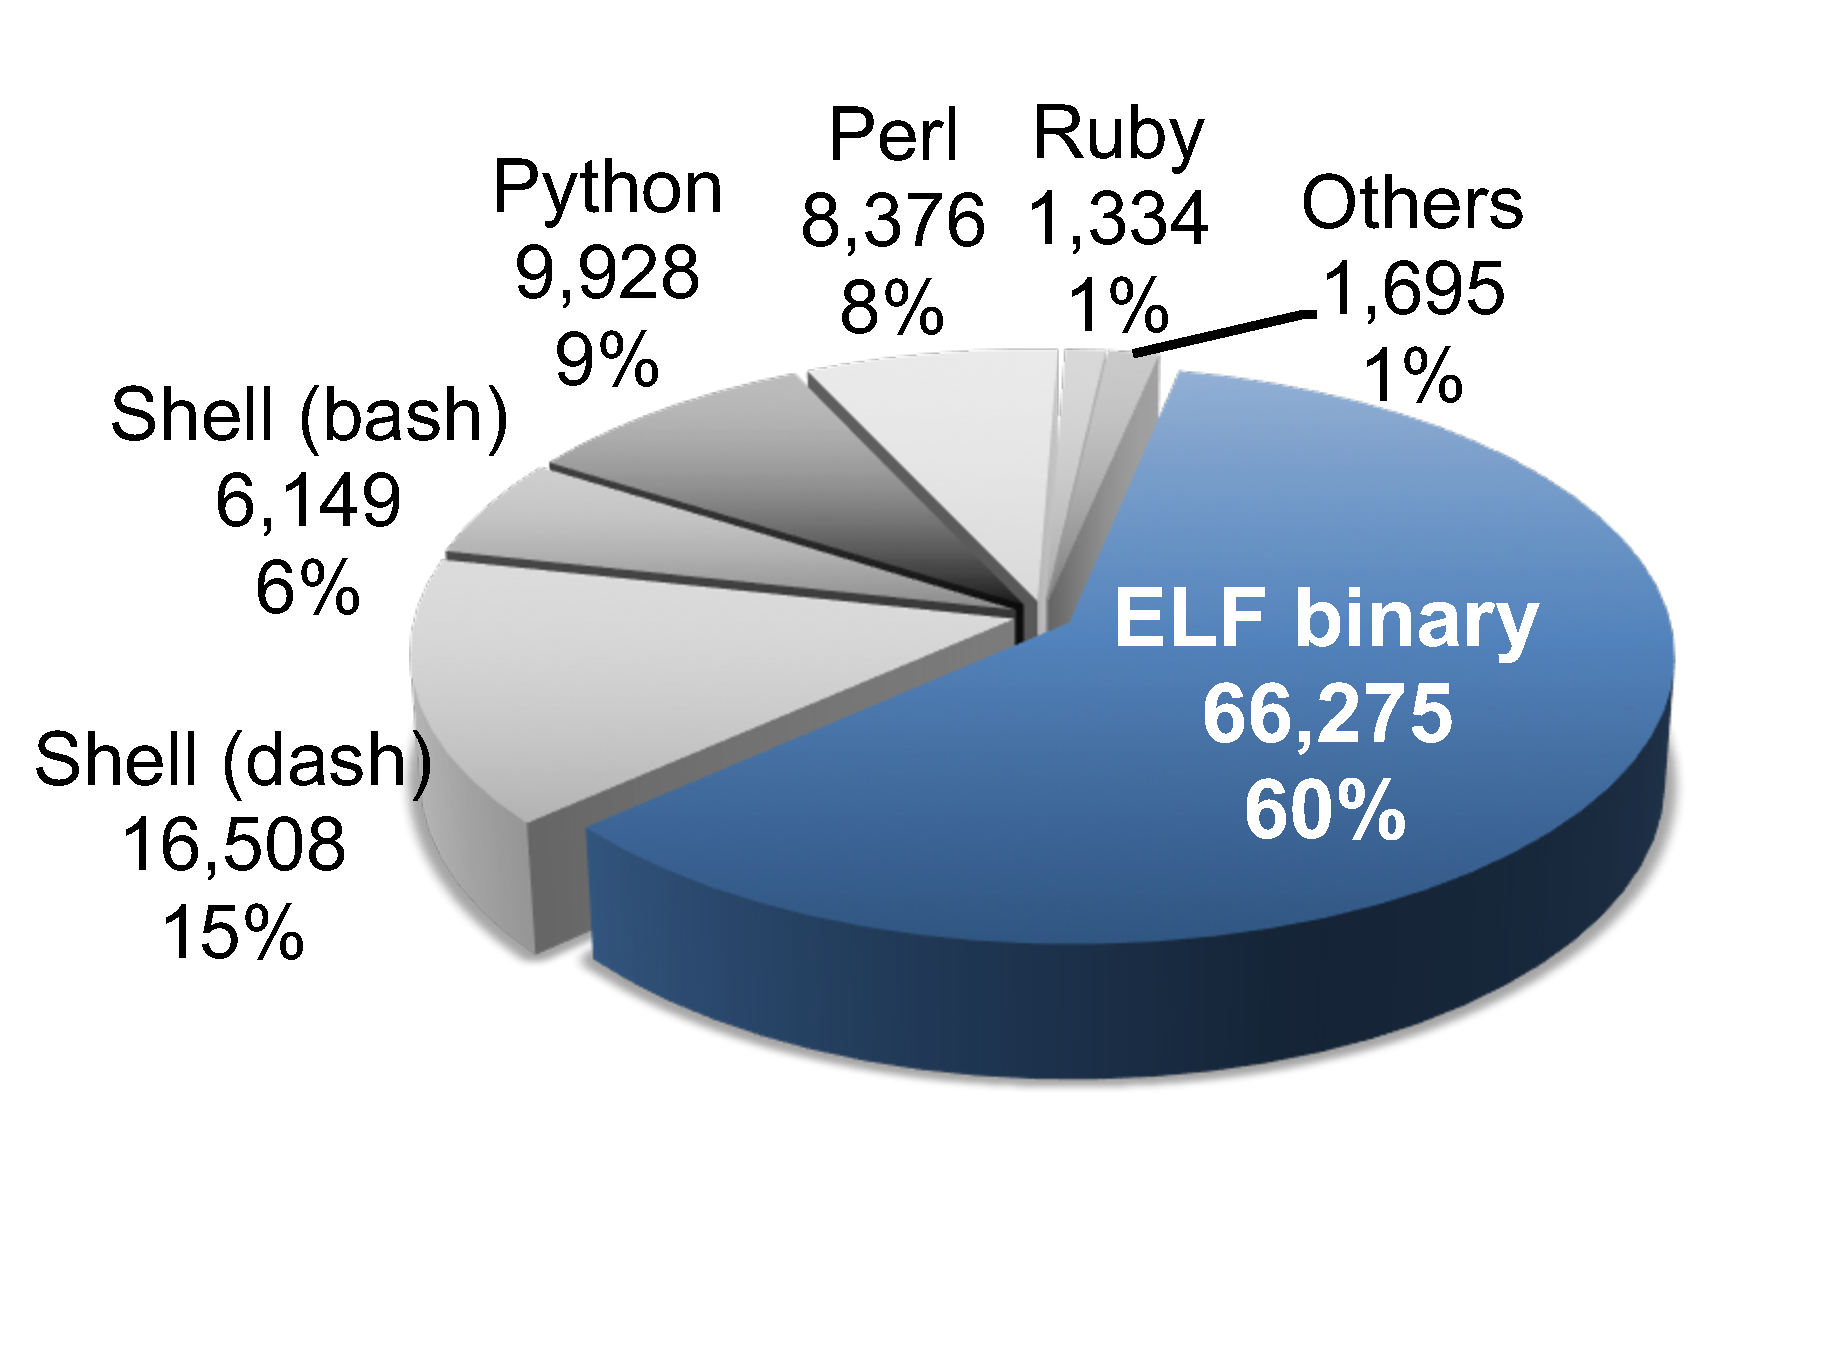
\includegraphics[width=3.2in]{syspop/figures/executable-type.pdf}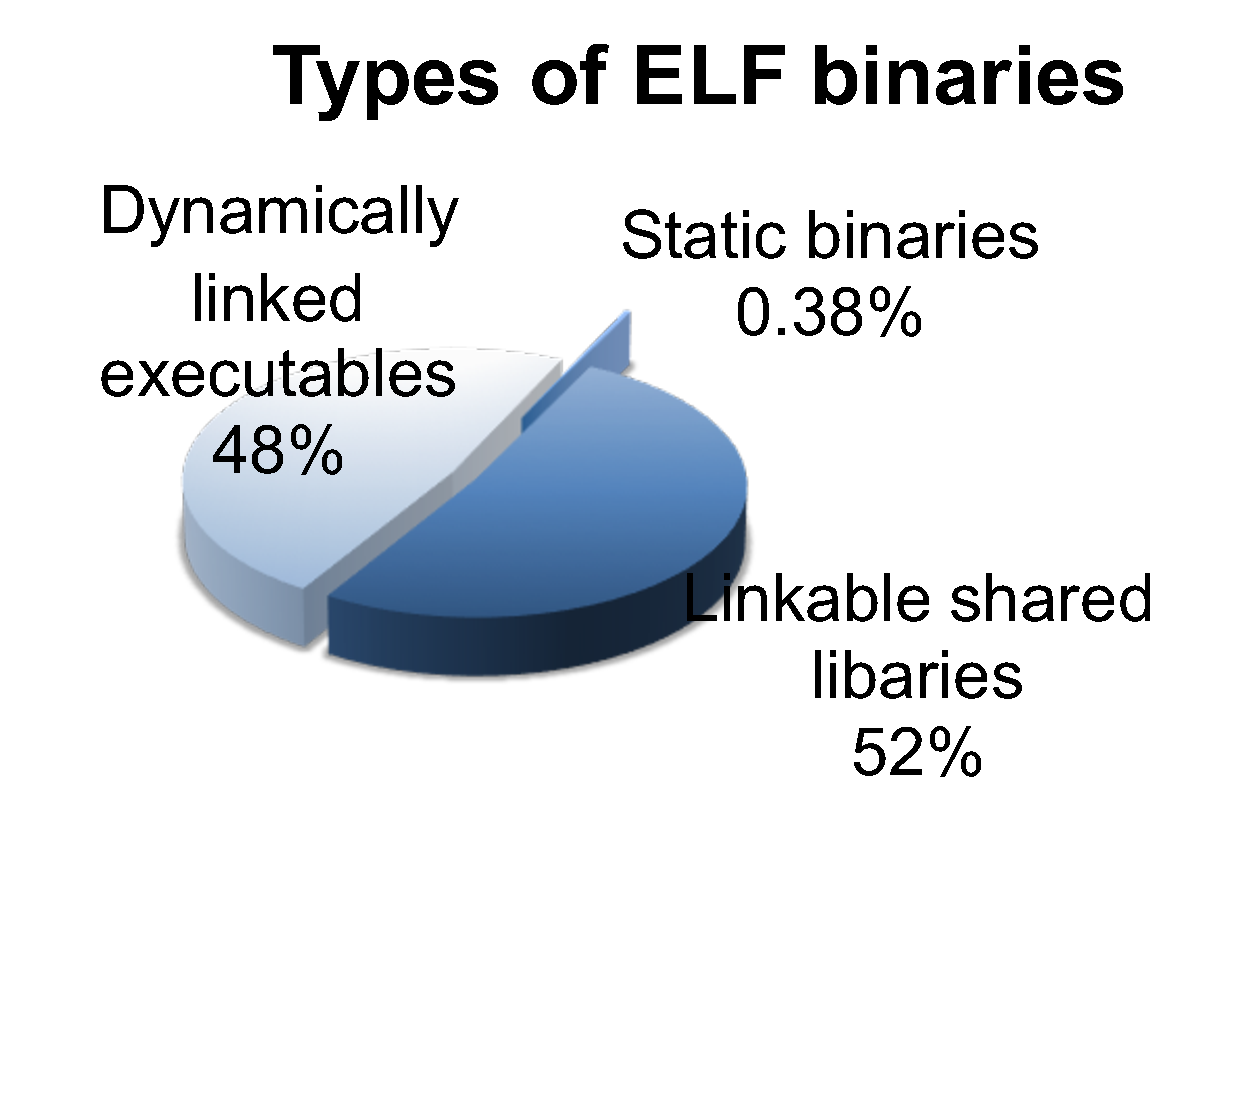
\includegraphics[width=2.4in]{syspop/figures/elf-binary-type.pdf}
\vspace{-0.5in}
\footnotesize
\caption[Types of executables included in the study of Linux API usage.]
{Percentage of ELF binaries and applications written in interpreted languages among all executables in the \osdist{} repository, categorized by interpreters. ELF binaries include static binaries, shared libraries and dynamically-linked executables. Interpreters are detected by {\em shebangs} of the files. Higher is more important.}
\label{fig:syspop:executable-type}
\end{figure}

Our study focuses primarily on ELF binaries, which account for the largest fraction of Linux applications
%which account for the plurality of Linux applications
(Figure~\ref{fig:syspop:executable-type}).
For interpreted languages, such as Python or shell scripts,
we assume that the system call footprint of the interpreter and major supporting libraries over-approximates the expected system call footprint of the applications.
Libraries that are dynamically loaded, such as application modules or
language native interface (e.g.,JNI, Perl XS) are not considered in our study. 
%\fixmedp{Does the analysis handle JNI, Perl XS, or other wrappers for native libraries?  I 
%could imagine the answer being yes if a .so is shipped, but possibly no 
%if it is somehow inlined}

%\fixmedp{Maybe move this up and merge with discussion above}

%% Similarly, there is a distinction between installation and regular use.  Ideally, one might filter applications
%% that were installed but never used, or have a second variant of \usagemetric{} that is weighted by frequency of use.
%% %Although we leave this for future work
%% However, we hasten to note that some infrequently-used applications are nonetheless important to users,
%% and frequency-independent metrics are still important.
%Similarly, there is a distinction between installation and regular use.
%Figure~\ref{fig:package-popularity} shows the trend of package installation statistics for the 500 most commonly installed packages.
%The \byinst{} data may {\it over-approximate} the \usagemetric{} of a package,
%whereas the \byvote{} may {\it under-approximate} important, but infrequently used packages.
%We err on the side of over-approximating \usagemetric{}, using \byinst{}
%weighting where not otherwise specified,
%although we present measurements based on both when appropriate.
%instead under-approximating is a safer strategy to quarantee the compatibility requirements to be fully deliverable.
%In this paper, we present measurements based on both \byinst{} and \byvote{} statisitcs to draw more observations.

%\begin{figure}[t!]
%\vspace{-0.1in}
%\center{
%\includegraphics[width=3.6in]{figures/package-popularity.pdf}
%}
%\footnotesize
%\vspace{-10pt}
%\caption{Package installation statisitics in \osdist{}, for 500 most installed packages managed by the repository. \byinst{} shows installations of packages. \byvote{} shows regularly used packages voted by installations. Higher is more popular.\fixmebj{Change the scale.}}
%\label{fig:package-popularity}
%\end{figure}

\subsection{Limitations}

%\fixmedp{Make sure we explain these:  the fact that the new metrics cannot distinguish between APIs that are critical to a small population, in that their functionality cannot be provided any other way, because they are new APIs not yet widely adopted, or because they are old APIs that are no longer used or were never used.}

\paragraph{Popularity Contest Dataset.}
The analysis in this paper is limited
by the \osdist{}'s package installer, \osinstaller{},
and their package installation statistics.
Because most packages in \osdist{} are open-source,
our observations on Linux API usage may have a bias toward open-source development patterns.
Commercial applications that are purchased and distributed
through other means are not included in this survey data,
although data from other sources could, in principle, be incorporated
into the analysis if additional data were available.
%the analysis can only be conducted manually,
%thus making it really hard to collect large amounts of samples.

We assume that the package installation statistics provided by \osdist{} are representative.
%The \osdist{} repository hosts \packagenum{} packages that contain application executables and libaries. 
The popularity contest dataset is reasonably large (\popsamples{} installations),
but reporting is opt-in.
Moreover,
%\fixmedp{check this para}
%The popularity contest dataset does not correlate 
%package installations, only shows how often each package is installed.
%Thus, we assume the installation of every package
%as an independent event, unless \osinstaller{} identifies the dependency otherwise.
the data does not show how often these packages
are actually used, only how often they are installed.
Finally, this data set does not include sufficient historical data
to compare changes to the API usage over time.


%% Another limitation of using
%% the package installation statistics
%% is that the statistics only show
%% the installation count of each package,
%% but no details about which packages each installation contains or
%% relative preferences among packages.
%% Therefore, our study must 




%% dp: This is covered elsehwere
%The usage statistics collected in this paper generate
%convincing observations and measurements for Linux-compatible platforms,
%due to the large-scale analysis of software packages in the \osdist{} repository.
%Although our analysis does not require source code,
%our resulting dataset is mostly focused on open-source applications.
%Only very few applications in the \osdist{} repositories are close-source,
%such as the Nvidia driver utilities.
%Our analysis only requires application binaries, and our resulting dataset covers 
%both open-source and closed-source applications. \fixmedp{Right?  Double check that do include some closed binaries}
%Because we focus on \osdist{} applications, and most are open-source (xx\% \fixmetsai{Need to find this number, it's not hard.}),
%the data may be biased toward open-source applications. 
%As a result, our observations on Linux API usage are largely biased toward open-source applications.
%Because the repositories for close-source applications
%are more scattered
%(even though they can be downloaded by \osinstaller{} if manually configured),
%it is hard to collect large amount samples about them.

%% Our study is focused on applications managed by \osinstaller{},
%% which are mostly open-source
%% (even though our approach requires no source code for analysis).

\paragraph{Static Analysis.}
Because our study only analyzes pre-compiled binaries, some compile-time customizations may be missed.
Applications that are already ported using macro like {\tt \#ifdef LINUX} will be considered dependent to Linux-specific APIs,
even though the application can be re-compiled for other systems.
Our static analysis tool only identifies 
whether an API is potentially used,
not how frequently the API is used during the execution.
Thus, it is not sufficient to draw inferences about performance.

%This study is only sufficient to draw conclusions or insight about compatibility, not about any impact on performance.
%The static analysis on application binaries only tells
%Also the package installation statistics provide no information
%about how often a package is used.
%This study cannot provide evidence for whether any APIs may dominate
%execution time.


%\note{Move this here}
We assume that, once a given API (e.g., {\tt write}) is supported and works for a reasonable sample of applications,
handling missed edge cases should be straightforward engineering that is unlikely to invalidate the experimental results of the project.
That said, in cases where an input can yield significantly different behavior, e.g.,
the path given to {\tt open},
we measure the \usagemetric{} of these arguments.
Verifying bug-for-bug compatibility generally requires techniques largely orthogonal to the ones used in this study,
and thus this is beyond the scope of this work.

We do not do inter-procedural data-flow analysis.  As a result,
we were unable to identify system call numbers for 2,454 call sites (4\% of the
relevant call sites)
across all binaries in the repository.  As a result,
some system call usage values may be underestimated, and may go up 
with a more sophisticated static analysis.


%% The package installation statistics provided by \osdist{}
%% show only information about how often packages are ``installed'',
%% not how often packages are ``used''.
%% Our study is based on an over-approximation of the actual package usage:
%% installed packages in any installation contain
%% at least the packages actually used.


\paragraph{Metrics.}
The proposed metrics are intended to be simple numbers for easy comparison.
But this coarseness loses some nuance. 
For instance, our metrics cannot distinguish between
APIs that are critical to a small population, such as those that offer 
functionality that cannot be provided any other way, 
versus APIs that are rarely used because the software is unimportant.
Similarly, these metrics alone cannot differentiate a new API 
that is not yet widely adopted from an old API with declining usage.


%% Although studying historical data may provide more insight about
%% how developer or user behaviors change, our approach requires more historical data to make any conclusions.
%% The installation statistics contain no version information,
%% so it is insufficient to determine the adoption time of any application changes.
%% For packages, \osinstaller{} only keeps the latest version of each package in each maintained snapshot.
%% The only way to backtrace all historical versions of a package
%% is to pull from a version-control repository maintained by the package developers, which may not always exist.

\section{Linux API Study}
\label{sec:syspop:study}

%\note{about 3 pages, include graphs}
%\note{try to break the page here so the whole observation can start on a new page}

%This section presents measurements of API usage,
%as well as several trends in how APIs are used. Of particular note is that
%the OS interface required by essentially all applications is 
%%the total OS interface that essentially all applications require is
%substantially larger than the roughly 300 Linux system calls---the required interface
%also includes several vectored system call operations, such as {\tt ioctl}, and special filesystem interfaces like {\tt /sys} and {\tt /proc}.
%We also note that a number of system calls and other APIs are so rarely used that they can be deprecated with little disruption or effort.
%
%This section first examines the use of system calls in Linux applications.
%Section~\ref{sec:observation:hello} analyzes the most efficient path to add system calls
%to a prototype, outlining a path from the minimal footprint for ``hello world'', 
%up through the most demanding application (qemu), maximizing the number
%of supported applications at each step.
%Section~\ref{sec:observation:vector} analyzes the importance of operations
%under vectored system calls, such as {\tt ioctl}.
%Section~\ref{sec:observation:pseudo} evaluates the \usagemetric{} of 
%pseudo-files, such as those under {\tt /proc}.
%Finally, Section~\ref{sec:observation:libc}
%examines current usage patterns for \libc{}.
%Throughout the section, we identify several points at which APIs could be gainfully
%restricted, removed, or refactored,
%as well as identifying points where unexpected APIs can be essential to performance or
%functionality.
%We highlight key insights and recommendations in boxes.

%% \rev{Explain the structure.}{In the following subsections,
%% we will discuss our findings on the API usage of different interface types,
%% followed by %boxed take-aways our quick tips (in double-framed boxes)
%% the lessons or insights in boxes.} 
%% \fixmedp{If a reviewer asked for a structure, I expect they want to know something like:
%% We first present system calls, then ioctls,
%% then pseudo file systems, etc.  In other words, what is the organizing principle for 
%% the following sub-sections?  Not that we discuss and then have a box} 

%\subsection{\usagemetric{} of Linux System Calls}
\subsection{System calls}
\label{sec:syspop:study:syscall}

%We begin by looking at the \usagemetric{} of each system call, 
%ordered by total application installations and regularly used applications 
%in order to answer the following questions:
%\begin{compactitem}
%\item Which system calls are the most important to support when implementing a new system,
%or have high costs to replace, if desired?
%%1) do we definitely need to support any of the surveyed systems?
%%2) are used by at least one frequently used application on the surveyed systems?
%\item Which system calls are very rarely used and candidates for deprecation?
%\item Which system calls are not supported by the OS, but still attempted by applications?
%\end{compactitem}
%\vspace{10pt}

There are \syscallnum{} system calls defined in \osarch{} Linux \kernelversion{} (as listed in {\tt unistd.h}). 
Figure~\ref{fig:syscall-popularity-trend} shows the 
distribution of system calls by importance.
The Figure is ordered by most important (at 100\%) to least important (around 0\%)---similar
to inverted CDF.
The figure highlights several points of interest on this line.

%The trends \byinst{} are useful to answer questions about supporting complete installations, 
%while the trends \byvote{} are useful to answer questions about supporting most popular 
%applications on most of the systems.
Over two-thirds ({\em 224 of \syscallnum{}}) 
of system calls on Linux are indispensable:
required by 
at least one application on every installation.
%only a little 
%over one-thirds ({\em 121 of \syscallnum{}}) of system calls are required 
%by at least one regularly used application (\byvote{}).
%\fixmedp{Would be nice to have more to say here, like filling out weighted compliance and the number of packages}
Among the rest, 33 system calls are important on more than ten percent of the installations.
44 system calls have very low \usagemetric{}:
less than ten percent of the installations include at least one application
that uses these system calls.
%Moreover, less than 10\% of the systems require 43 system calls.
%and 58 system calls are regularly used on less than 10\% of the systems (\byvote{}).
%For instance, {\tt timer\_delete}, {\tt timer\_create} and {\tt timer\_settime} are used by 
%at least one application on all the systems, however, the applications using these 
%system calls are regularly used only on 17\% of the systems. 
%Another system call 
%{\tt tkill} used by {\tt strace} installed ubiquitously on all systems 
%is used regularly only on 3\% of the systems. So, even if the installation statistics imply that 
%{\tt tkill} needs to be supported to support at least one of the machines,
%only 3\% of those machines regularly use that system call.

Our study also shows the contributors
to an API's importance. %\usagemetric{}.
For instance, Table~\ref{tab:syspop:wrapped} lists system calls that are
only called by one or two particular libraries
(e.g., \libc{}).
These system calls are wrapped by library APIs,
so applications depend on them only because the libraries do.
To eliminate the usage of these system calls,
developers only have to pay minimum efforts to re-implement the wrappers in libraries.

\begin{figure}[t]
\centering
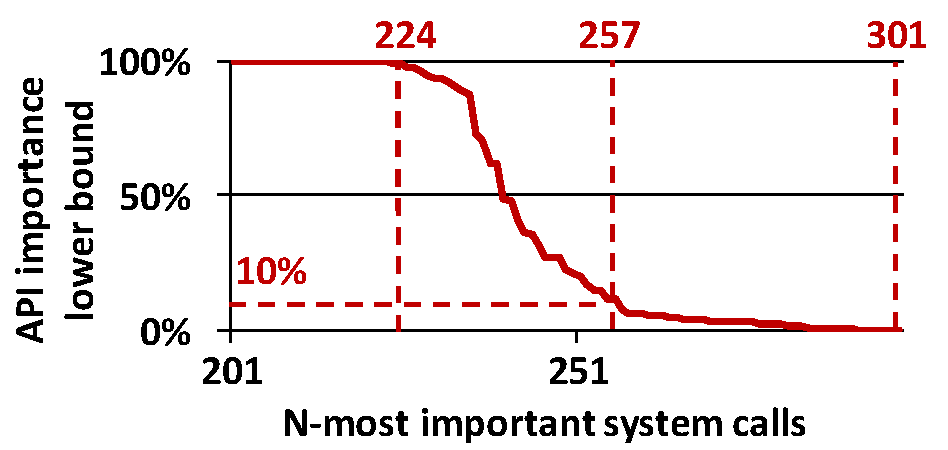
\includegraphics[width=\textwidth]{syscall-popularity-all-by-inst.pdf}
\caption[N-most important system calls in Linux.]
{The trend of \usagemetric{} as N-most important system calls among total \syscallnum{} system calls of \osversion{} with Linux kernel \kernelversion{}. .
Higher is more important; 100\% indicates all installations include software that make the system call.}
\label{fig:syscall-popularity-trend}
\end{figure}

%\callout{It is easy to support regularly used parts of an installation than complete installations of the surveyed systems.} 

Among the 44 system calls with a \usagemetric{} above zero but less than ten percent,
some are cases where a more popular alternative is available.
%developers appear more motivated by 
%portability than security.
%, the bottom 20 non-zero are listed in Table~\ref{tab:syscall-popularity-bottom}, along with the packages that use these interfaces.
%%11 of the bottom 20 system calls are Linux-specific.
%%This shows that portability to other Unix variants
%%has a significant effect on adoption.
%%bP: These conclusions cannot be made with weighted importance.
For instance, Linux supports both POSIX and System V message queues.
The five APIs for POSIX message queues have a lower
\usagemetric{} than System V message queues.
We believe this is attributable to System V message queues %provide a better designed interface, they
being more portable to other UNIX systems.
%they are not adopted by most popular applications.}
Similarly, we observed that {\tt epoll\_wait} (100\%) has a higher \usagemetric{} than {\tt epoll\_pwait} (3\%),
even though {\tt epoll\_pwait} is commonly considered more robust
for the same purpose---waiting on file descriptor events.
Table~\ref{tab:dominated} lists
system calls used by only one or two packages---generally special-purpose utilities,
such as {\tt kexec\_load}, which is used by {\tt kexec-tools}).
%,These system calls are mostly used by special-purpose utilities (e.g., 
%and generally address  because their semantics are not friendly enough.

\begin{table}[t!b!]
  \centering
  \small
  \begin{tabular}{>{\footnotesize\raggedright\arraybackslash}p{1.45in} >{\raggedleft\arraybackslash}p{0.25in}>{\raggedright\arraybackslash}p{1.15in}}
\toprule
{\bf System Calls} & {\bf Imp.} & {\bf Packages}\\
\midrule
{\tt clock\_settime}, {\tt iopl}, {\tt ioperm},  {\tt signalfd4}  & 100\% & libc \\
{\tt mbind}             & 36.0\% & libnuma, libopenblasp \\
{\tt addkey}            & 27.2\% & libkeyutils \\
{\tt keyctl}            & 27.2\% & pam\_keyutil, libkeyutils \\
{\tt requestkey}        & 14.4\% & libkeyutils \\
{\tt preadv}, {\tt pwritev}   & 11.7\% & libc \\
    \end{tabular}%
   \caption{System calls which are only directly used by particular libraries, and their \usagemetric{} (``Imp.''). Only system calls with \usagemetric{} larger than ten percent are shown.
These system calls are wrapped by library APIs,
thus they are easy to deprecate by modifying the libraries.  
}
  \label{tab:wrapped}%
\end{table}%

\begin{table}[t!b!]
\centering
\small
\begin{tabular}{>{\palign[\footnotesize]{l}}p{2.9in} >{\palign{r}}p{1.1in}>{\palign{l}}p{2in}}
\toprule
{\bf System Calls} & {\bf \UsageMetric{}} & {\bf Used Packages}\\
\midrule
{\tt seccomp}, {\tt sched\_setattr}, {\tt sched\_getattr}  & 1\% & coop-computing-tools \\
\hline
{\tt kexec\_load} & 1\% & kexec-tools \\
\hline
{\tt clock\_adjtime} & 4\% & systemd \\
\hline
{\tt renameat2} & 4\% & systemd, coop-computing-tools \\
\hline
{\tt mq\_timedsend}, {\tt mq\_getsetattr} & 1\% & qemu-user \\
\hline
{\tt io\_getevent} & 1\% & ioping, zfs-fuse \\
\hline
{\tt getcpu} & 4\% & valgrind, rt-tests \\
\hline
\end{tabular}%
\caption[System call usage dominated by particular package(s)]
{System calls with usage dominated by particular package(s), and their \usagemetric{}. This table excludes system calls that are officially retired.}
\label{tab:dominated}%
\end{table}%


In some cases, system calls are effectively offloaded to a file in {\tt /proc} or {\tt /sys}.
For instance, some of the information that was formerly available via 
{\tt query\_module} can be obtained from {\tt /proc/modules}, {\tt /proc/kallsyms} 
and the files under the directory {\tt /sys/module}. Similarly, the information that can be obtained from the {\tt sysfs} system call
is now available in {\tt /proc/filesystems}.

%We found five  API that have very low 
%compared to the System V message queue API.

We also found five system calls {\tt uselib}, {\tt nfsservctl}, {\tt afs\_syscall}, {\tt vserver} and {\tt security} system calls that are officially retired, but still have a low, but non-zero, \usagemetric{}. 
For instance {\tt nfsservctl} is removed from Linux kernel 3.1 but
still has \usagemetric{} of seven percent,  %\fixmedp{Do we have some examples of apps that use it?}
because it is tried by NFS utilities such as {\tt exportfs}.
These utilities still attempt the old calls for backward-compatibility with older kernels.
%Application maintainers of packages using these retired system calls need to be notified to port their applications to support latest kernel.


%\callout{System developers can use our framework to actively notify relevant package maintainers while retiring system calls.} 
%\callout{Among 43 least-used system calls, some are replaceable
%by alternatives with higher \usagemetric{};
%5 are officially retired but still tried by few applications.
%System developers could use this data to identify relevant applications,
%accelerating replacement of these system calls.}




\begin{table}[t!b!]
\centering
\small
\begin{tabular}{>{\palign[\footnotesize]{l}}p{.5\textwidth} >{\palign{l}}p{.45\textwidth}}
\toprule
\textbf{Unused System Calls} & \textbf{Reason for Disuse}\\
\midrule
{\footnotesize
{\tt set\_thread\_area}, {\tt tuxcall}, {\tt create\_module}, and 7 more. } & Officially retired.\\
\hline
{\tt sysfs} & replaced by {\tt /proc/filesystems}.\\
\hline
{\tt rt\_tgsigqueueinfo}, {\tt get\_robust\_list} & Unused by applications.\\
\hline
{\tt remap\_file\_pages} & No non-sequential ordered mapping; repeated calls to mmap preferred.\\
\hline
{\tt mq\_notify} & Unused: Asynchronous message delivery.\\
\hline
{\tt lookup\_dcookie} & Unused: for profiling.\\
\hline
{\tt restart\_syscall} & Transparent to applications.\\
\hline
{\tt move\_pages} & Unused: for NUMA usage. \\
\hline
\end{tabular}%
\caption{Unused system calls and explanation for disuse.}
\label{tab:syspop:unused}%
\end{table}%



%On the other end of the spectrum, 

In total, 18 of \syscallnum{} system calls in Linux \kernelversion{} are not used by any application in the \osdist{} repository. We list these system calls in Table~\ref{tab:syspop:unused}.
In addition to the issues discussed above,
Ten of these system calls do not have an entry point, but are still defined in the Linux headers.
%\fixmedp{Why are they in the count then?  do you mean 320 defined system call numbers}
%Similarly, we analyze the 21 system calls with 0 \usagemetric{} as shown in 
%Table~\ref{tab:unused}. 
%{\tt sysfs} is replaced by alternate interface {\tt /proc/file\linebreak[0]systems}.
%%On the other hand, even though {\tt remap\_file\_pages} system call was added to map pages of a file into memory in a non-sequential order since Linux version 2.6 (in 2003), no application is actually using it. This indicates that either no application is mapping pages in non-sequential order or applications are repeatedly using the more popular generic system call like {\tt mmap}.
%Similarly, {\tt mq\_notify} system call for receiving asynchronous notification about new messages in message queue is not used, because \usagemetric{} of message queue interfaces is less than 5\% in the first place and applications using message queue do not use asynchronous communication.
Five of the unused system calls such as {\tt rt\_tgsig\linebreak[0]queueinfo}, {\tt get\_robust\_list}, {\tt remap\_\linebreak[0]file\_pages}, {\tt mq\_notify}, {\tt lookup\_dcookie} provide an interface that is not used by the applications. These system calls can be potential candidates for deprecation.
However, even though {\tt restart\_\linebreak[0]syscall} is not used by any application, it is internally used by the kernel. % transparent to userspace.
%Finally, 4 NUMA related system calls are not used 
%\rev{rewrite}{because none of our samples is written to be NUMA-aware}.
%\fixmetsai{Check if libnuma uses these system calls.}

%\callout{In addition to ten already retired system calls, we found seven other candidate system calls for deprecation or in need of more exposure to developers.}

\begin{comment}
\begin{table}[t]
\center{
\footnotesize
\begin{tabular}{m{0.45\linewidth}m{0.45\linewidth}}
\hline
Syscalls & Packages\\
\hline
process\_vm\_writev & coop-computing-tools, care, proot, stress-ng \\
vserver & util-vserver\\
syncfs & ceph-test, ploop, ruby-passenger, ceph\\
io\_getevents & ioping, zfs-fuse\\
uselib & mupdf, mupdf-tools\\
afs\_syscall & openafs-fileserver, openafs-kpasswd, openafs-krb5, openafs-client, openafs-dbserver\\
kexec\_load & kexec-tools\\
mq\_getsetattr, mq\_timedsend & qemu-user, qemu-user-static\\
vmsplice & criu, qemu-user-static, fio, stress-ng, qemu-user\\
timer\_gettime & ben, galax-extra, libocamlnet-ocaml-bin, ocsigenserver, galax, approx, qemu-user-static, galaxd, matita, cduce, qemu-user, turnserver, stress-ng\\
timerfd\_gettime & ben, approx, libocamlnet-ocaml-bin, ocsigenserver, openclonk, matita, galax, galaxd, qemu-user-static, galax-extra, cduce, qemu-user\\
eventfd & blktap-utils, julia, nodejs\\
semtimedop & tgt, dahdi, gtk-gnutella, prayer, libopenni-sensor-primesense0, libopenni-sensor-pointclouds0\\
timer\_getoverrun & emacs24-lucid, emacs24, qemu-user-static, qemu-user, emacs24-nox, rt-tests, reconserver, miredo\\
mq\_timedreceive & qemu-user-static, nilfs-tools, xjadeo, rt-tests, qemu-user\\
acct & watchdog, acct, qemu-user-static, qemu-user, scm, atop\\
fanotify\_init, fanotify\_mark & fatrace, fnotifystat, health-check, clamav-daemon\\
open\_by\_handle\_at & qemu-system-mips, qemu-system-misc, qemu-system-sparc, qemu-system-ppc, qemu-system-arm, qemu-system-x86\\
\hline
\end{tabular}
}
\footnotesize
\caption{20 system calls with the lowest \usagemetric{} among 297 used system calls in \osversion{} with Linux Kernel \kernelversion{}, except the ones with \usagemetric{} lower than 0.01\% (considered negligible).}
\label{tab:syscall-popularity-bottom}
\end{table}
\end{comment}

\begin{comment}
There are 43 system calls with low non-zero \usagemetric{} of less than 10\%.
%, the bottom 20 non-zero are listed in Table~\ref{tab:syscall-popularity-bottom}, along with the packages that use these interfaces.
%%11 of the bottom 20 system calls are Linux-specific.
%%This shows that portability to other Unix variants
%%has a significant effect on adoption.
%%bP: These conclusions cannot be made with weighted importance.
We found 5 POSIX message queue API that have very low 
\usagemetric{} compared to the System V message queue API because 
even if POSIX message queues provide a better designed interface, they are less 
widely available. We also found 5 system calls {\tt uselib}, {\tt nfsservctl}, {\tt afs\_syscall}, {\tt vserver} and {\tt security} system calls that are officially retired, and have non-zero albeit negligible \usagemetric{}. 
For instance {\tt nfsservctl} is removed from Linux kernel 3.1 but
still has \usagemetric{} of 7\%. Application maintainers of packages using these retired system calls need to be notified to port their applications to support latest kernel.
Also, we observed that {\tt epoll\_wait} (100\%) has more \usagemetric{} than {\tt epoll\_pwait} (3\%)
even though {\tt epoll\_pwait} is safer to use to wait for a file descriptor to become available.
In some cases, system calls are effectively offloaded to a file in {\tt /proc} or {\tt /sys}.
For instance, some of the information that was formerly available via 
{\tt query\_module} can be obtained from {\tt /proc/modules}, {\tt /proc/kallsyms} 
and the files under the directory {\tt /sys/module}. Also same information obtained from {\tt sysfs} is
also available from {\tt /proc/filesystems}.

\callout{System developers can use our framework to actively notify relevant package maintainers while retiring system calls.} 
\end{comment}

%%% \begin{figure}[H]
%%% \center{
%%% \includegraphics[height=1.1in]{figures/syscall-popularity-top-1.pdf}
%%% \hspace{-0.3in}
%%% \includegraphics[height=1.1in]{figures/syscall-popularity-top-2.pdf}
%%% }

%%% \begin{minipage}[t]{\linewidth}
%%% \scriptsize
%%% \vspace{-0.1in}
%%% \setlength{\parindent}{-0.2in}
%%% \setlength{\leftskip}{0.2in}
%%% {\bf * Top-1:} \hspace{0.1in}(195 system calls) \hspace{0.1in}\usagemetric{} = 1.0000\\
%%% {\tiny\tt
%%% read,write,open,close,stat,polllseek,mmap,brk,rt\_sigprocmask,ioctl,access,pipe,select,shmget,nanosleep,socket,clone,vfork,kill,
%%% etc.
%%% }

%%% \vspace{0.1in}
%%% {\bf * Top-2:} \hspace{0.1in}(8 system calls) \hspace{0.1in}\usagemetric{} = 0.9999\\
%%% {\tiny\tt
%%% reboot,timer\_create,iopl,getitimer,accept4,
%%% etc.
%%% }
%%% \end{minipage}
%%% \footnotesize
%%% \caption{20 groups of system calls with the highest \usagemetric{} among 279 used system calls in \osversion{} (Linux Kernel \kernelversion{})}
%%% \label{fig:syscall-popularity-top}
%%% \end{figure}

%\begin{figure}[H]
%\center{
%\includegraphics[height=1.15in]{figures/syscall-popularity-bottom.pdf}
%}
%\footnotesize
%\caption{20 system calls with the lowest \usagemetric{} among 279 used system calls in \osversion{} (Linux Kernel \kernelversion{}), except the ones with \usagemetric{} lower than 0.0001 (considered negligible).\fixmedp{Convert to table}}
%\label{fig:syscall-popularity-bottom}
%\end{figure}

%\subsection{From ``Hello World'' to Qemu}
%\label{sec:observation:hello}

Figure~\ref{fig:syscall-compatibility} shows the optimal path of adding system calls to a prototype system,
using a simple, greedy strategy of implementing the N-most important APIs, which in turns
maximizes \compatmetric{}.
In other words, the leftmost points on the graph are the most important APIs,
but the y coordinate only increases once enough system calls
are supported that a simple program, such as ``hello world'' can execute. %\fixmedp{Right?}
Similar to a CDF, this line
continues up to 100\% of Ubuntu applications.  The graph highlights several 
points of interest in this curve.

Essentially, one cannot run even the most simple programs without at least 40 system calls.
After this, the number of additional applications one can support by adding another system call increases
steadily until an inflection point at 125 system calls, or supporting extended attributes on files,
where \compatmetric{} jumps to 25\%.
To support roughly half of \osdist{} applications, one must have 145 system calls, and
the curve plateaus around 202 system calls.  
On the most extreme end, qemu's MIPS emulator (on an \osarch{} host) requires 270 system calls~\citep{Bellard05}.
A \compatmetric{} of 100\% implies that
%all Linux system calls
all Linux applications ever used
are supported by the prototype.

\begin{figure}[t]
\centering
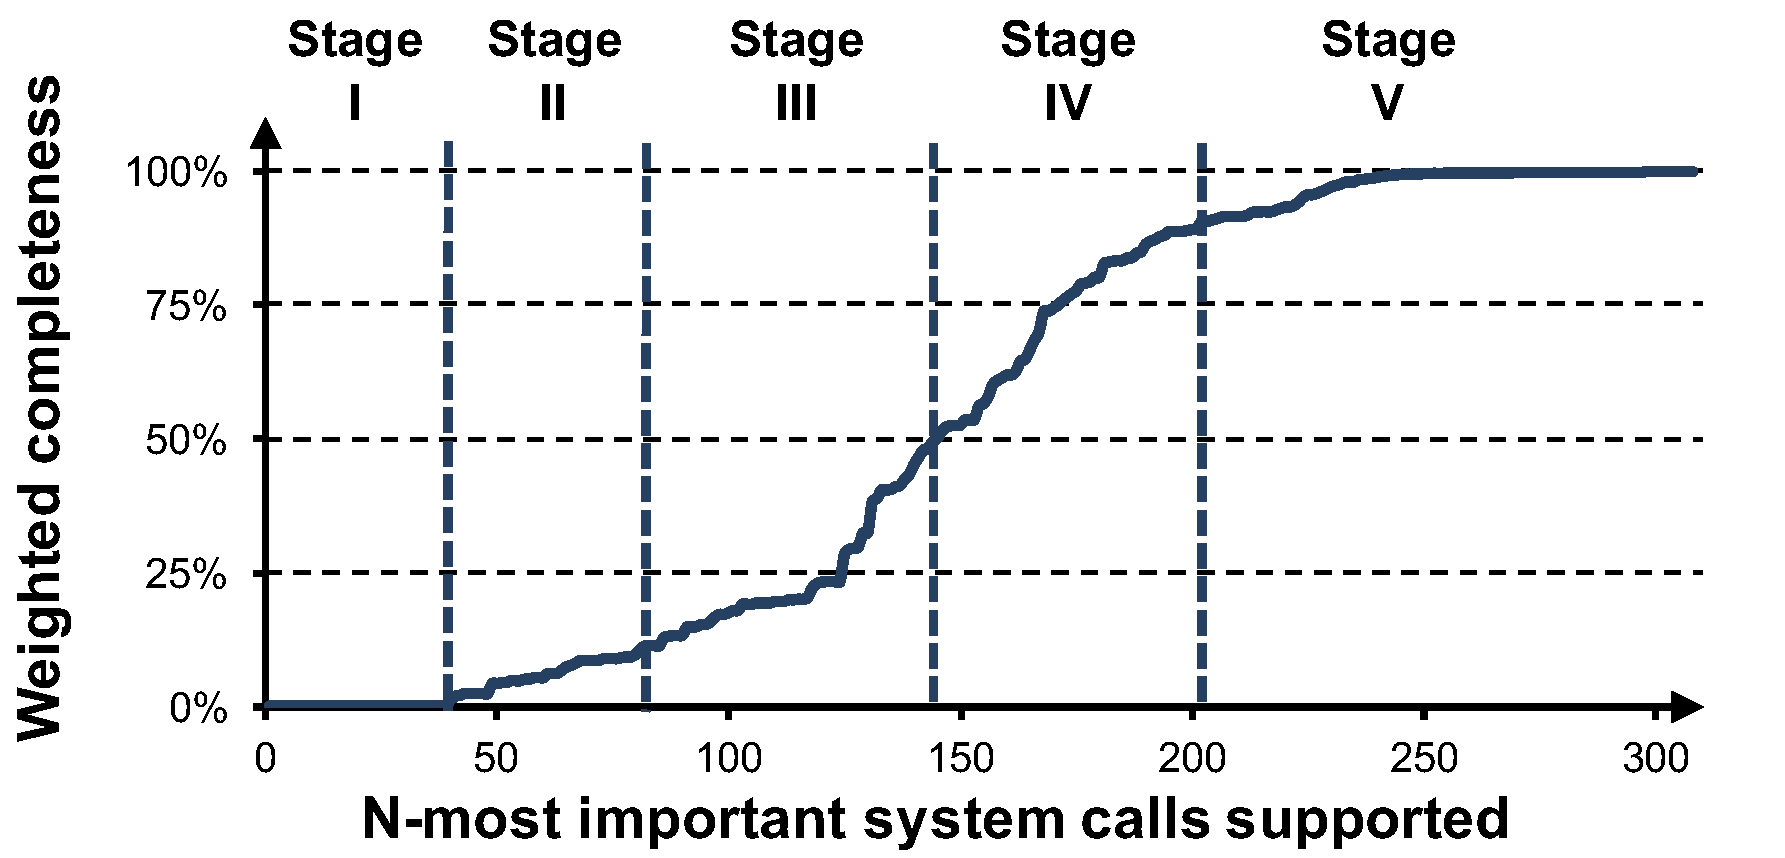
\includegraphics[width=.8\textwidth]{syscall-compatibility.pdf}
\caption{Accumulated \compatmetric{} when N top-ranked system calls are implemented in the OS. Higher is more compliant.}
\label{fig:syscall-compatibility}
\end{figure}

\begin{table}[t]
\center{
\begin{tabular}{c>{\footnotesize\raggedright\arraybackslash}m{.5\textwidth}>{\raggedleft}m{.15\textwidth}>{\raggedleft\arraybackslash}m{.15\textwidth}}
\toprule
Stage & {\normalsize Sample System Calls} & \# syscalls & {\footnotesize \CompatMetric{}} \\
\addlinespace
\midrule
I &
{\tt mmap}, {\tt vfork}, {\tt exit}, {\tt read},
{\tt gettid}, {\tt fcntl}, {\tt getcwd}
{\tt sched\_yield}, {\tt kill}, {\tt dup2}
& 40 & 1.12 \% \\
\midrule
II &
{\tt mremap}, {\tt ioctl}, {\tt access}, {\tt socket},
{\tt poll}, {\tt recvmsg}, {\tt dup},
{\tt unlink}, {\tt wait4}, {\tt select}, {\tt chdir}, {\tt pipe}
& +41 (81) & 10.68 \% \\
\midrule
III &
{\tt sigaltstack}, {\tt shutdown}, {\tt symlink},
{\tt alarm}, {\tt listen}, {\tt pread64}, {\tt getxattr}, 
{\tt shmget}, {\tt epoll\_wait},
{\tt chroot}
& +64 (145) & 50.09 \% \\
\midrule
IV &
{\tt flock}, {\tt semget}, {\tt ppoll},
{\tt mount}, {\tt brk}, {\tt pause},
{\tt clock\_gettime}, {\tt getpgid}, {\tt settimeofday},
{\tt capset}
& +57 (202) & 90.61 \% \\
\midrule
V & {\normalsize All remaining} & +70 (272) & 100 \% \\
\bottomrule
\end{tabular}
}
\footnotesize
\caption[Proposed steps of Linux system call implemetation prioritzed by importance]
{Five stages of implementing system calls based on the \usagemetric{} ranking. For each stage, a set of system calls is listed, with the work needed to accomplish (\# of system calls) and the \compatmetric{} that can be reached.}
\label{table:syscall-stage}
\end{table}

Table~\ref{table:syscall-stage} breaks down the recommended development phases by rough categories of required system calls.
We do not provide a complete ordered list here in the interest of brevity, but this list is available as part of our dataset, 
at \projecturl{}.

A goal of \compatmetric{} is to help guide the process of developing new system prototypes.
Section~\ref{sec:observation:syscall} showed that 224 out of \syscallnum{} system calls on \osdist{} have 100\% \usagemetric{}.
In other words, if one of these 224 calls is missing, at least one application on a typical system will not work.
\Compatmetric{}, however, is more forgiving, as
it tries to capture the fraction of a typical installation that could work.
Only 
40 system calls are needed to have \compatmetric{} more than 1\%.
%However, to achieve non-zero \compatmetric{} to \osdist{}, it does not require a system to support all 226 system calls;
%only 
%% The reason of such a gap is that \usagemetric{} is
%% a metric more sensitive to the API usage of individual applications:
%% as long as at least one application in every installation uses
%% a specific API, its \usagemetric{} will be 100\%.
%% \compatmetric{} is a metric made relatively relaxed:
%% this metric evaluates the expected fraction of any installation that can be supported,
%% to provide meaningful measurements

%\callout{It takes the most effort to support first and last 10\%
%of any installation (0--10\% and 90--100\% \compatmetric{}).
%The gain in functionality is precipitous when adding the 81st--202nd system calls.}

For simplicity, Table~\ref{table:syscall-stage}
only includes system calls, % \compatmetric{} based on system ,
but one can construct a similar path including other APIs, % the metric also considers other APIs,
such as vectored system calls, pseudo-files and library APIs.
For example, developers need not implement every operation of
{\tt ioctl}, {\tt fcntl} and {\tt prctl}
during the early stage of developing a system prototype.
%\fixmedp{Would it make sense to do this after the ioctls and files are covered, and include important ioctls and files?  Also, check my rewrite}

%\fixmedp{This callout is not really justified by the text  I took the point to be that the right 132 and 202 system calls are ``sweet spots'' on the path to maturity.}

\subsection{Vectored System Calls}
\label{sec:syspop:study:vector}

%\fixmedp{I think RD is right: can we give more landscape of what the long tail of vectored calls are for?  Why do they exist?}

Some system calls, such as {\tt ioctl}, {\tt fcntl},
and {\tt prctl}, essentially export a secondary system call table, 
using the first argument as an operation code.
These {\it vectored} system calls significantly expand the system API, 
dramatically increasing the effort to realize full API compatibility.
%and essentially make it harder to implement a compatibility layer.
It is also difficult to enforce robust security policies on these interfaces,
as the arguments to each operation are highly variable.
%\fixmedp{Can we comment on what, say SELinux or AppArmor actually do with ioctl?}


The main expansion is from {\tt ioctl}.
Linux defines 635 operation codes, and 
Linux kernel modules and drivers can define additional operations.
In the case of {\tt ioctl}, we obverse that there are 52 operations with the 100\% \usagemetric{} (Figure~\ref{fig:syspop:opcode-popularity}),
each of which are as important as the 226 most important system calls.
Of these 52 operations,  47 are frequently used operations for TTY console (e.g., {\tt TCGETS}) or generic operations on IO devices (e.g., {\tt FIONREAD}).

%A narrow vectored system call like {\tt fcntl} has eighteen operations in , and {\tt prctl} has 44 operations so far.
%A wider vectored system call like 
%which are further 



On the narrow end, {\tt fcntl} and {\tt prctl} have 18 and 44 operations, respectively, in Linux kernel \kernelversion{}.
Unlike {\tt ioctl}, {\tt fcntl} and {\tt prctl} are not extensible by modules or drivers,
and their operations tend to have higher \usagemetric{} (Figure~\ref{fig:syspop:opcode-popularity}).
For {\tt fcntl}, eleven out of eighteen {\tt fcntl} operations in Linux \kernelversion{} have \usagemetric{} at around 100\%.
For {\tt prctl}, only nine out of 44 operations have \usagemetric{} around 100\%,
and only eighteen has \usagemetric{} larger than 20\%.
%Because of the more equally important operations, {\tt fcntl} is a less urgent target for reformation, while {\tt prctl} has plenty of unused or infrequently used read-only operations that can be moved to pseudo-file system interfaces like {\tt /proc}.


Thus, developers of a new system prototype should support these 47 most important {\tt ioctl}
operations, about half of the {\tt fcntl} opcodes, and only 9--20 {\tt prcntl} operations.


%% Although the 47-most important ioctl operations have 100\% \usagemetric{},
%% promoting any of these operations to system calls is not beneficial.
%% Vectored system calls with limited amounts of operation codes
%% are almost equally easy to secure and maintain
%% as normal system calls.
%% However the disruptiveness of removing these operations codes
%% is unbearable for applications. 

%% However, knowing the most important operations for vectored system calls,
%% developers of new system prototypes can choose to
%% implement only part of these vectored system calls to obtain significant improvement on \compatmetric{}.
%% %For instance, Graphene library OS~\citep{tsai14graphene} only implements {\tt FIONREAD} of {\tt ioctl} to satisfy the most common usage in applications. 

%\callout{In building a prototype system, a relatively small set of operations
%in vectored system calls are essential.}
%Highly important operations in vectored system calls
%can be implemented first, to achieve better \compatmetric{}
%with partial support of these system calls.}}

%These operations are candidates for promotion to standalone system calls,
%for better usability, more attention for their security, and ease of filtering.  

%\callout{The most ubiquitous vector operations should be upgraded to system calls.}


Compared to system calls, 
{\tt ioctl} has a much longer tail of infrequently used operations.
Out of 635 {\tt ioctl} operation codes defined by modules or drivers hosted in Linux kernel \kernelversion{},
only 188 have \usagemetric{} more than one percent,
and for only 280 we can find usage of the operations in at least one application binary.
Those unused operations are good targets for deprecation, in the interest
of reducing the system attack surface.
%since leaving them around causes the OS open to attacks if any vulnerabilities exist in these APIs.
%\fixmetsai{What can we find out in this long tail?}

%\callout{{\tt ioctl} system call has a very long tail of unused operations, which may create system security risks.}

\begin{figure}[t]
\centering
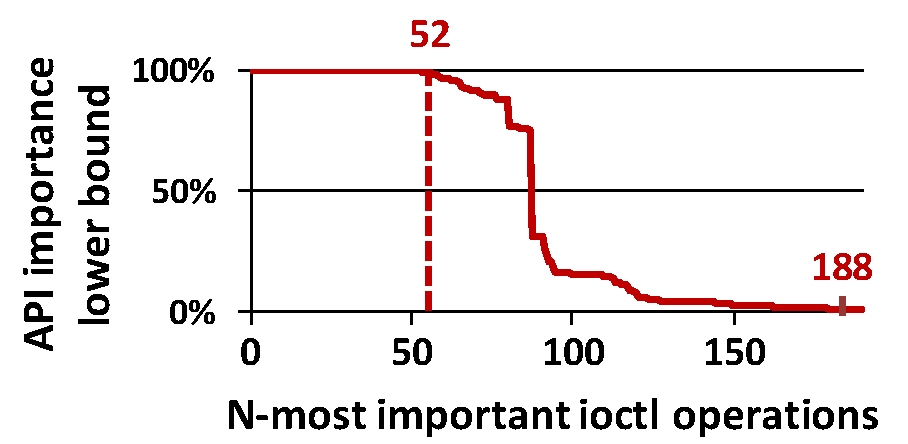
\includegraphics[width=.48\textwidth]{ioctl-popularity-by-inst.pdf}
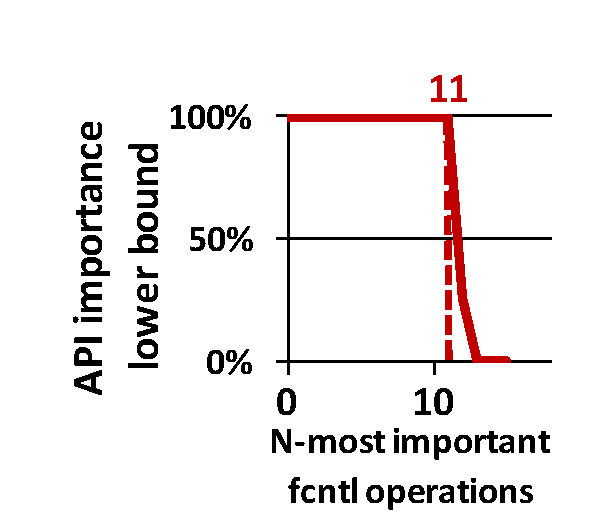
\includegraphics[width=.25\textwidth]{fcntl-popularity-by-inst.pdf}
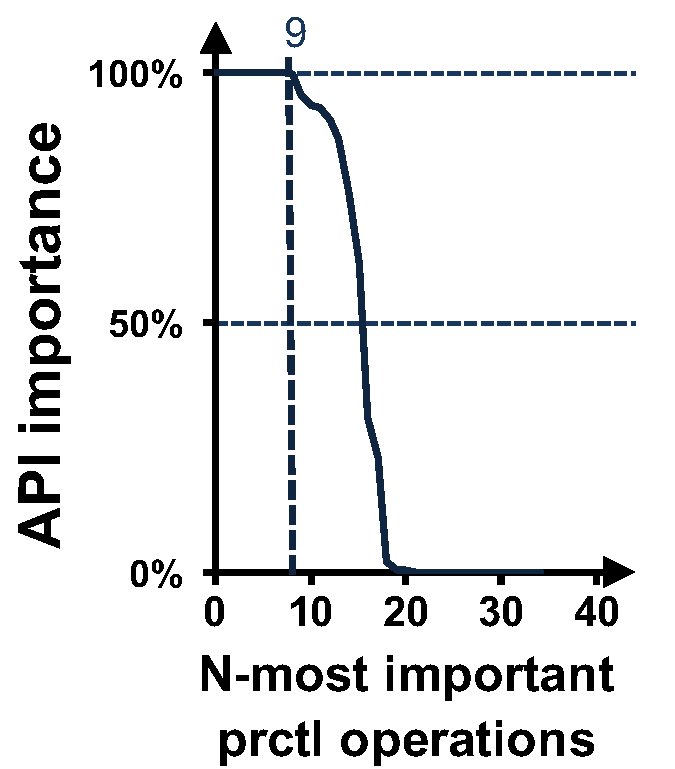
\includegraphics[width=.25\textwidth]{prctl-popularity-by-inst.pdf}
\caption{Ranking of \usagemetric{} among {ioctl}, {\tt fcntl} and {\tt prctl} opcodes.  Higher is more important; 100\% indicates all installations include software that request the operations.}
\label{fig:syspop:opcode-popularity}
\end{figure}


%\fixmedp{If time, it would be nice to investigate these zero cases and make sure no one really uses them}

%\begin{figure}[t]
%\center{
%\includegraphics[width=0.95\linewidth]{figures/fcntl-popularity.pdf}
%}
%\footnotesize
%\caption{Ranking of \usagemetric{} among {\tt fcntl} commands.}
%\label{fig:fcntl-popularity}
%\end{figure}

%\begin{figure}[t]
%\center{
%\includegraphics[width=0.95\linewidth]{figures/prctl-popularity.pdf}
%}
%\footnotesize
%\caption{Ranking of \usagemetric{} among {\tt prctl} codes.}
%\label{fig:prctl-popularity}
%\end{figure}

\subsection{Pseudo-Files and Devices}
\label{sec:syspop:study:pseudo}

In addition to the main system call table, Linux exports many additional APIs through 
pseudo-file systems, such as {\tt /proc}, {\tt /dev}, and {\tt /sys}.
These are called pseudo-file systems because they are not backed by disk, but
rather export the contents of kernel data structures to an application or administrator
as if they were stored in a file.
These pseudo-file systems are a convenient location to export tuning parameters, statistics, 
and other subsystem-specific or device-specific APIs.
Although many of these pseudo-files are used on the command line or in scripts by an administrator,
a few are routinely used by applications.
% interfaces are often the last resort of APIs, for accommodation of the most exotic interfaces. 
In order to fully understand usage patterns of the Linux kernel, pseudo-files must also be considered.

We apply static analysis to find cases where the binary is hard-coded to use a pseudo-file.
Our analysis cannot capture cases where a path to one of these file systems is passed as 
an input to the application, such as {\tt dd if=/dev/zero}.
However, when a pseudo-file is widely-used as a replacement for a system call,
these paths tend to be hard-coded in the binary as a string or string pattern.
%most instances of these file systems as system call replacements have hard-coded paths or patterns 
%in the binary.  
A common pattern we observed was {\tt sprintf(``/proc/\%d/cmdline'', pid)}; our analysis captured these patterns as well.
We also do not differentiate types of access in this study, such as separating read
versus write of a pseudo-file; rather we only consider whether the file is accessed or not.
Thus, our analysis is limited to strings stored in the binary, but we believe this captures
an important usage pattern.  %is a reasonable sample.


%% Note that matching hard-coded paths in binaries does not differentiate
%% the type of access on the files or devices.
%% The possible access on a pseudo file includes reading or writing data, retrieving file attributes, waiting on file descriptor events,
%% or performing directory operations.
%% Our study treat all access to one particular pseudo-file or device
%% as using the same API.

\begin{figure}[t]
\centering
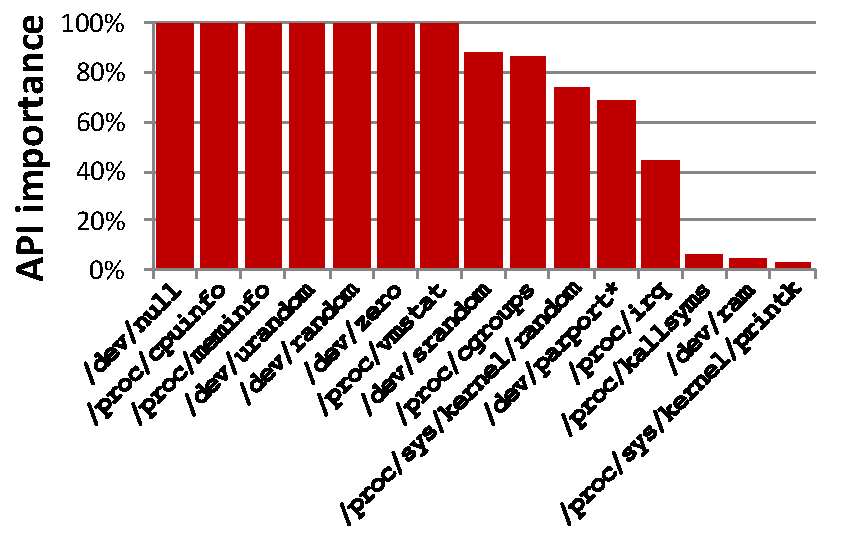
\includegraphics[width=5.5in]{syspop/figures/dev-proc-popularity-by-inst.pdf}
\caption{\usagemetric{} distribution over files under {\tt /dev} and {\tt /proc}.  Higher is more important; 100\% indicates all installations include software that accesses the file. }
\label{fig:syspop:dev-proc-popularity}
\end{figure}

Figure~\ref{fig:syspop:dev-proc-popularity} shows the \usagemetric{} of common pseudo-files under {\tt/dev} and {\tt /proc}.  
These files are ordered from highest \usagemetric{}; the long tail
of files used rarely or directly by administrators is omitted.

%There are two striking facets of this data.
Some files %under {\tt /proc} and {\tt /dev}
are essential,
such as {\tt /dev/null} and {\tt /proc\-/\-cpuinfo}.
These files are widely used in %are hard to deprecate because the usage of
%these APIs exists in not only 
binaries and scripts.
%\fixmedp{Can we comment on how many apps or libraries include a hard-coded string or pattern?}
Among 12,039 binaries that use a hard-coded path,
3,324 access {\tt /dev/null} and 439 access {\tt /proc/cpuinfo}.
However, it is plausible to provide the same functionality in
simpler ways.
For instance, {\tt /proc/cpuinfo} provides a formatted wrapper for
the {\tt cpuinfo} instruction, which one could export
directly to userspace using virtualization hardware, similar to Dune~\citep{belay12dune}.
Similarly, {\tt /dev/zero} or {\tt /dev/null} are convenient for use on the command
line, but it is surprising that a significant number of applications
issue {\tt read} or {\tt write} system calls, rather than simply zeroing a buffer
or skipping the {\tt write}
(e.g., {\tt grub-install}).
%\fixmedp{Can we offer concrete examples of apps that do this?}
Thus, in implementing a Linux compatibility layer, a small number of pseudo-files
are essential, and perhaps others could be eliminated with modest application changes.


%% provide more security-aware alternatives
%% to these APIs, so security-sensitive applications
%% can remove the usage to reduce their attack surfaces.}
%% %These system calls can be either repromoted to system call interfaces,
%% %or directly served inside system libraries using a library OS approach,
%% %to avoid increasing API footprint.
%% For example, \libc{} can encapsulate {\tt /dev/null} and serve it in the user space.
%% %without the usage of real system calls.
%% {\tt /proc/cpuinfo} can be stored as a static information in user's memory,
%% or retrieved from CPU using the {\tt CPUINFO} instruction.

APIs as pseudo-files or pseudo-devices also have a large subset
of infrequently used or unused APIs.
%Second, pseudo-file systems contain a large collection of APIs that are infrequently used,
Many of them
are designed to support one specific application or user.
%only serve certain special purposes for few applications or end-users
For example, {\tt /dev/kvm} is only intended for {\tt qemu} to
communicate with the kernel portion of the KVM hypervisor.
Similarly {\tt /proc/kallsyms} is used primarily to export debugging information to kernel developers.

Because so many files in {\tt /proc} are accessed from the command line
or by only a single application, it is hard to conclude that any should be deprecated.
Nonetheless, these files represent large and complex APIs that create an important attack surface to defend.
As noted in other studies, the permission on {\tt /proc} tend to be
set liberally enough to leak a  significant amount of information~\citep{memento}.
%\fixmedp{Can we comment on how many of these are really accessible from regular applications/ how used in SELinux/AppArmor}
For files used by a single application, an abstraction like a fine-grained capability~\citep{shapiro99eros}
might better capture this need.  
%\fixmedp{I think kvm actually does use some sort of capability already. Please check.}
For files used primarily by the administrator,
carefully setting directory permissions should be sufficient.
%, but with careful consideration of using any security-enhanced Linux variant.



%% Although cleaning up the unused APIs is beneficial for the cleanness of the system design,
%% because pseudo-files and pseudo-devices are often considered
%% the last resort of APIs,
%% developers may choose not to deprecate them.
%% %there is no reason to deprecate them or delegate them to other interfaces
%% %if OS maintainers still consider the APIs useful.
%% %For example, {\tt /proc/kallsyms}
%% %only has \usagemetric{} less then ten percent,
%% %but it is
%% %a necessary API for Linux kernel development.
%% Instead of deprecating unused API,
%% we can apply more secure mechanisms, such as AppArmor or SELinux,
%% to restrict the access to particular applications.}
%% %to prevent them from becoming system vulnerabilities. 

%\callout{A few pseudo-files are essential and must be implemented
%by any Linux-emulator.  Most serve a specific purpose, and might benefit
%from stricter enforcement of the principle of least privilege.}

%For pseudo-files and devices that are ubiquitously important, system developers should provide more secure alternatives
%if possible. Infrequently used APIs that are important for particular applicatins need to be further secured.}}

%First, the \usagemetric{} of these file under {\tt /proc} is very bimodal.
%There are over 1,000 files that are not directly used by any application; we expect that most of these
%are interfaces for an administrator to adjust kernel behavior.

%Second, there are 148 files with an \usagemetric{} score above 90\%---almost as many as there are system calls with a similar \usagemetric{} score.

%\fixme{Remove the discussion about performance impact for now. Will resurrect it after I confirm it is true.}
%In some cases, libraries or applications can tolerate a missing {\tt /proc} file
%by falling back to default values or alternate interfaces.
%For instance, {\tt gcc} will try to read {\tt /proc/cpuinfo} to guide its selection of optimizations and {\tt /proc/meminfo} to avoid
%swapping; if this file is not available, 
%{\tt gcc} will use default values.
%Our static analysis does not detect these cases.
%Nonetheless, in building a Linux-compatibility system, whether these pseudo-files are accurately 
%emulated can have a first-order impact on performance.
%In our experience building the Graphene library OS~\citep{tsai14graphene}, {\tt gcc}
%performance \fixmedp{data nugget here}.

%developers interested in emulating Linux or similar systems should carefully evaluate their emulation of {\tt /proc}.

In the case of the {\tt /dev} file system, the most commonly used files are pseudo-devices, such as accessing
the virtual terminal ({\tt /dev/tty}, {\tt /dev/console}, and {\tt /dev/pts}), or other functionality 
such as the random number generator ({\tt /dev/urandom}).
Even among pseudo-devices, features such as accessing one's standard in and out, or a process's TTY
via the {\tt /dev/} interface are not heavily used.

Intuitively, one would not expect many device paths to be hard-coded, and most direct interactions 
with a device would be done using administrative tools.
For instance, we see that some applications do hard-code paths like {\tt /dev/hda} (commonly used for an IDE hard drive),
yet an increasing number of systems have a root hard drive using SATA, which would consequently be named {\tt /dev/sda}.
Thus, although applications may use paths like {\tt /dev/hda} as a default device path, modern systems are sufficiently varied
that these generally need to be searched at runtime.

%\begin{figure}[t]
%\centering
%\includegraphics[width=0.9\linewidth]{figures/sys-popularity.pdf}
%\caption{\usagemetric{} distribution over the set of files under {\tt /%sys}.  Higher is more heavily used; 1 indicates all systems include %software that accesses the file. }
%\label{fig:sys-popularity}
%\end{figure}

%In the case of {\tt /sys} (Figure~\ref{fig:sys-popularity}), 
%we again note that there are 63 paths with a \usagemetric{} value above 90\%,
%and a total of 97 above 20\%.  Several of these export CPU or power management features,
%or user-accessed buses, like USB.  Unlike {\tt /dev}, several of these hard-coded files 
%are also actual (expected) devices, such as PCMCIA devices.

%Table~\fixmedp{XX} lists the {\tt /proc} files with a \usagemetric{} score of one.  
%\fixmedp{What else to say about this?  Might be more interesting to know how ubiquitously used these are}

\subsection{\Libc{} functions}
\label{sec:syspop:study:libc}

In addition to studying kernel interfaces, we also analyze the \usagemetric{} of APIs
defined in core system libraries, such as \libc{}.
Most programmers don't directly use the APIs exported by the kernel,
but instead program to more user-friendly APIs in \libc{} and other libraries.
%The \libc{} implementation contains lots of wrappers,
%or more user-friendly API variants of system calls and others.
For instance, \glibc{}~\citep{glibc} exports APIs for using locks and condition variables, which internally 
use the subtle {\tt futex} system call~\citep{franke02futex}.

%Figure~\ref{fig:syspop:libc-popularity} 
Our result shows that among %shows the \usagemetric{} of 
the global function symbols exported by 
\libc{} --- 1,274 in total % API among all packages. 
%Here we define \libc{} API as functions that are exported as global function symbols in \libc{}.
%The definition yields a total of 1,274  APIs,
%Among these APIs,
--- 42.8\% have a \usagemetric{} of 100\%,
50.6\% have a \usagemetric{} of less than 50\%,
and 39.7\% have a \usagemetric{} of less than one percent, including some that are not used at all.
In other words, about 40\% of the APIs inside \libc{}
are either not used or only used by few applications.
This result implies that most processes are loading a significant amount of 
unnecessary code into their address space.
By splitting \libc{} into several sub-libraries, based on \usagemetric{}
and common linking patterns, systems could realize a non-trivial space savings.

%\fixmedp{Can we assert that important and unimportant APIs are interleaved
%  on the same pages, so lazy loading doesn't help?}
There are several reasons to avoid loading extra code into an application.
First, there are code reuse attacks, such as return-oriented programming (ROP)~\citep{return-oriented},
that rely on the ability to find particular code snippets, called gadgets.
Littering a process with extra gadgets offers needless assistance to an attacker.
Similarly, when important and unimportant APIs are on the same page,
memory is wasted.  
Finally, the space overhead of large, unused jump tables is significant.
In \glibc{} 2.21, {\tt libc-2.21.so} essentially has 1274 relocation entries, occupying 30,576 bytes of virtual memory. 
%\fixmedp{true?: Because important and unimportant APIs are interleaved, all of these pages typically demand-allocated, even for applications that only use the most popular entries.}
By sorting the relocation table according to API usage,
most \libc{} instances could load only first few pages of relocation tables, and leave the remaining relocation entries for lazy loading.

We analyzed the space savings of a 
\glibc{} 2.21 which removed any APIs with \usagemetric{} lower than 90\%.
In total, \libc{} would retain 889 APIs
and the size would be reduced to 63\% of its original size.
%to \libc\_minor (in total  will stay in \libc{}).
%The size of \libc{} is reduced to 
The probability an application would need a missing function and load it from another library is less than 9.3\%(equivalent to 90.7\% \compatmetric{} for the stripped \libc{}).
%and the probability of any application loading \libc\_minor is smaller than 9.3\% 
Further decomposition is also possible, 
such as placing APIs
that are commonly accessed by the same application into the same sub-library.

%% Knowing the usage of \libc{} APIs, developers can decompose
%% a large \libc{} binary into smaller libraries.
%% Breaking down the size of \libc{} binary effectively reduces
%% the security threats in \libc{},
%% such as the risk of ROP (Return-Oriented Programming) attack.
%% The simplest way of decomposing \libc{} is
%% to move all APIs with lower \usagemetric{}
%% to another library \libc\_minor.


%It could reduce effective memory footprint to deprecate the functions that are never used, 
%or move rarely-used APIs into a separate library. % additional libraries so they do not have to be loaded or installed all the time.

%% \rev{Transition}{Another minor benefit of decomposing \libc{}
%% or just re-ordering \libc{} APIs
%% is to optimize the resource usage needed for dynamic loading of these APIs.}
%% %Other usage of this statistics is to provide them to compilers as a hint to optimize the dynamic loading.
%% Dynamic libraries like \libc{} are relocated during loading time
%% of user processes,
%% and the virtual memory used for storing relocation tables for
%% all libraries loaded in all user processes can be a non-trivial memory footprint because they are unable to share physical pages.
%% In \glibc{} 2.21, {\tt libc-2.21.so} essentially has 1274 relocation entries, occupying 30,576 bytes of virtual memory. 
%% By sorting the relocation table according to API usage,
%% Most \libc{} can load only first few pages of relocation tables, and leave the remaining relocation entries for lazy loading.

%\callout{Decomposing or re-ordering library API can lower memory costs
%in typical application processes.}
%API usage statistics are hints for compilers to optimize memory footprint of dynamic loading by sorting relocation tables by \usagemetric

%\begin{figure}[t]
%\centering
%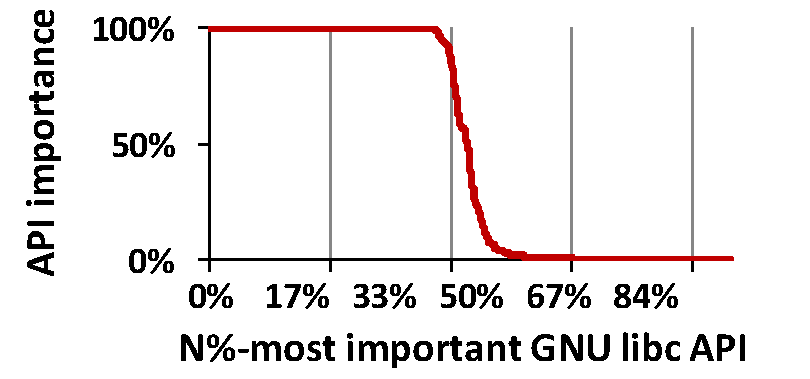
\includegraphics[width=3.6in]{syspop/figures/libc-popularity.pdf}
%\caption[\Usagemetric{} distribution of GNU Library C functions]
%{\usagemetric{} distribution over the set of GNU Library C. Higher is more important; 100\% indicates all installations include software that use the \libc{} API. }
%\label{fig:libc-popularity}
%\end{figure}

%%%We observe that majority (xx \%) of the executables in the \osdist{} repository are ELF binaries (Figure~\ref{fig:executable-type}).
%%%The other executables rely on interpreters like shell, perl, python, etc. We focus our study
%%%only on the ELF binaries which also include the interpreters for other scripts. However, we do
%%%not use the scripts popularity and their footprint while calculating the metric for system call popularity.
%%%Overall, in order to get a compatibility score with Linux for any given OS, we calculate popularity of 4 different
%%%interfaces that the applications use.

\paragraph{Effects of standard libraries on \usagemetric{}.} \Libc{} and the dynamic linker ({\tt ld.so}) 
also contribute to the system call footprint of every dynamically-linked executable.
This has a marked effect on the \usagemetric{} of some system calls.
The APIs used to initialize a program  are listed in Table~\ref{table:libc-init-call}.
In several cases, such as {\tt set\_tid\_address}, however, \libc{} or \libpthread{} may be the only binaries using these interfaces directly,
indicating that changes to some important system interfaces would only require changes in one or two low-level libraries.

%\callout{GNU Library C and the dynamic linker can have a first-order effect on the \usagemetric{} of some system calls.}

%%% \begin{compactenum}
%%% \item Users and developers are often unaware of the footprint caused inside initialization and finalization of \libc{}. For library APIs, users at least have basic sense about what the footprint may look like.
%%% \item It requires only minimal effort to maintain compatibility between GNU Library C and kernel, because the development is actually closely coupled. 
%%% \end{compactenum}
 

%%% These APIs are also the fundamental API footprint of a {\tt Hello World} program.
%%% The developers of GNU C library made the choice of relying on certain APIs, making them one of the most important in the system. 

%%% For example, in our study, the usage in \libc{} has increased the \usagemetric{} of system call {\tt set\_tid\_address} by 0.75, suggesting that deprecating the system call will takes only little effort but changing {\em libc} itself.    

\begin{table}[t]
\centering
\small
\begin{tabular}{>{\footnotesize\raggedright\arraybackslash}m{.6\textwidth}>{\raggedright\arraybackslash}m{.3\textwidth}}
\hline
\addlinespace
System Calls & Libraries \\
\addlinespace
\hline
{\tt access}, {\tt arch\_prctl}, {\tt mprotect} & ld.so \\
\hline
{\tt clone}, {\tt execve}, {\tt getuid}, {\tt gettid},
{\tt kill}, {\tt getrlimit}, {\tt setresuid} & libc \\
\hline
{\tt close}, {\tt exit}, {\tt exit\_group}, {\tt getcwd},
{\tt getdents}, {\tt getpid}, {\tt lseek}, {\tt lstat},
{\tt mmap}, {\tt munmap}, {\tt madvise}, {\tt mprotect},
{\tt mremap}, {\tt newfsstat}, {\tt read} &
libc, ld.so \\
\hline
{\tt rt\_sigreturn}, {\tt set\_robust\_list}, {\tt set\_tid\_address} &
libpthread \\
\hline
{\tt rt\_sigprocmask} &
librt \\
\hline
{\tt futex} &
libc, ld.so, libpthread \\
\hline
\end{tabular}
\footnotesize
\caption{Ubiquitous system call usage caused by initialization or finalization of \libc{} family.}
\label{table:libc-init-call}
\end{table}

\section{System Evaluation}

This section uses \compatmetric{} to evaluate systems or emulation layers with partial Linux compatibility.
We also evaluate several \libc{} variants for their degree of completeness against the APIs exported by \glibc{} 2.21.

\subsection{Linux compatibility layers}

\begin{table}[t]
\centering
\small
\begin{tabular}{m{.3\textwidth}>{\centering}m{.05\textwidth}>{\raggedright\arraybackslash\footnotesize}m{.4\textwidth}>{\raggedleft\arraybackslash}m{.15\textwidth}}
\toprule
Systems & \# & Suggested APIs to add & \Compatmetric{} \\
\midrule
\addlinespace
User-Mode-Linux \kernelversion{} & 284 & {\tt name\_to\_handle\_at}, {\tt iopl}, {\tt perf\_event\_open} & 93.1\% \\
\addlinespace
\hline
\addlinespace
L4Linux 4.3 & 286 & {\tt quotactl}, {\tt migrate\_pages}, {\tt kexec\_load} & 99.3\% \\
\addlinespace
\hline
\addlinespace
FreeBSD-emu 10.2 & 225 & {\tt inotify}*, {\tt splice}, {\tt umount2}, {\tt timerfd}* & 62.3\% \\
\addlinespace
\hline
\addlinespace
Graphene  & 143 & {\tt sched\_setscheduler}, {\tt sched\_setparam} & 0.42\% \\
Graphene\textsuperscript{\P} & 145 & {\tt statfs}, {\tt utimes}, {\tt getxattr}, {\tt fallocate}, {\tt eventfd2} & 21.1\% \\
\hline
\end{tabular}
\caption{\Compatmetric{} of several Linux systems or emulation layers. For each system, we manually identify the number of supported system calls (``\#''), and calculate the \compatmetric{} (``W.Comp.'') . Based on \usagemetric{}, we suggest the most important APIs to add.
(*: system call family.
\P: Graphene after adding two more system calls.) }
\label{tab:linux-compat}
\end{table}

To evaluate the \compatmetric{} of Linux systems or emulation layers,
the prerequisite is to identify the supported APIs of the target systems.
Due to the complexity of Linux APIs and system implementation,
it is hard to automate the process of identification.
However, OS developers are mostly able to maintain such a list based on the internal knowledge. 

We evaluate the \compatmetric{} of four Linux-compatible systems or emulation layers:
User-Mode-Linux~\citep{user-mode-linux}, L4Linux~\citep{hartig97mu}, FreeBSD emulation layer~\citep{freebsd-emu}, and Graphene library OS~\citep{tsai14graphene}.
For each system, we explore techniques
to help identifying the supported system calls,
based on how the system is built.
For example, User-Mode-Linux and L4Linux
are built by modifying the Linux source code,
or adding a new architecture to Linux.
These systems will define architecture-specific system call tables,
and reimplement {\tt sys\_*} functions in the Linux source
that are originally aliases to {\tt sys\_ni\_syscall}
(a function that returns {\tt -ENOSYS}). 
Other systems, like FreeBSD and Graphene,
are built from scratch,
and often maintain their own system call table structures,
where unsupported systems calls
are redirected to dummy callbacks.

%Because the evaluation is simply a proof-of-the-concept,
%we count only system calls,
%omitting other APIs such as vectored system calls and pseudo-files. 

Table~\ref{tab:linux-compat} shows \compatmetric{},
considering only system calls.
The results also identify the most important system calls
that the developers should consider adding. 
User-Mode-Linux and L4Linux both have a \compatmetric{} over 90\%,
with more than 280 system calls implemented.
FreeBSD's  \compatmetric{} is  62.3\% because it is missing some less
important system calls
such as {\tt inotify\_init} and {\tt timerfd\_create}.
Graphene's \compatmetric{} is only 0.42\%.
We observe that the primary culprit is 
scheduling control; by adding two scheduling system calls,
Graphene's \compatmetric{} would be 21.1\%.

\subsection{Standard C libraries}

\begin{table}[t]
\center{
\small
\begin{tabular}{>{\raggedright\arraybackslash}m{.25\textwidth}>{\raggedleft\arraybackslash}m{.05\textwidth}>{\raggedright\arraybackslash\footnotesize}m{.25\textwidth}>{\raggedleft\arraybackslash}m{.15\textwidth}>{\raggedleft\arraybackslash}m{.15\textwidth}}
\toprule
\Libc{} variants & \# & Unsupported functions (samples) & {\footnotesize \Compatmetric{}} & {\footnotesize \Compatmetric{}} {\scriptsize (normalized)} \\
\midrule
\addlinespace
eglibc 2.19 & 2198 & None & 100\% & 100\% \\
\addlinespace
\hline
\addlinespace
uClibc 0.9.33 & 1867 & {\tt \_\_uflow}, {\tt \_\_overflow}  & 1.1\% & 41.9\% \\
\addlinespace
\hline
\addlinespace
musl 1.1.14 & 1890 & {\tt secure\_getenv}, {\tt random\_r} & 1.1\% & 43.2\% \\
\addlinespace
\hline
\addlinespace
dietlibc 0.33 & 962 & {\tt memalign}, {\tt stpcpy}, {\tt \_\_cxa\_finalize}  & 0\% & 0\% \\
\addlinespace
\hline
\end{tabular}
}
\caption{\Compatmetric{} of \libc{} variants. For each variant, we calculate \compatmetric{} based on symbols directly retrieved from the binaries,
and the symbols after reversing variant-specific replacement (e.g.,\funcname{printf} becomes \funcname{\_\_printf\_chk}).}
\label{tab:libc-compat}
\end{table}

This study also uses \compatmetric{} to evaluate the compatibility of several \libc{} variants --- eglibc~\citep{eglibc}, uClibc~\citep{uclibc}, musl~\citep{musl} and dietlibc~\citep{dietlibc} --- against \glibc{},
listed in Table~\ref{tab:libc-compat}.
We observe that, if simply matching exported API symbols, only eglibc is directly compatible to \glibc{}.
Both uClibc and musl have a low \compatmetric{}, because \glibc{}'s headers replace a number of APIs with safer variants at compile time, using macros.
For example, \glibc{} replaces {\tt printf} with {\tt \_\_printf\_chk}, which performs an additional check for stack overflow.
%Because these new APIs often have the same interface as the old ones,
%we assume other \libc{} variants can easily
%reverse the API replacement during symbol resolution.
After normalizing for this compile-time API replacement, both uClibc and musl are at over 40\% \compatmetric{}.
In contrast, dietlibc is still not compatible with most binaries linked against \glibc{} --- if no other approach is taken to improve its compatibility.
The reason of low \compatmetric{} is that dietlibc does not implement many ubiquitously used \glibc{} APIs such as {\tt memalign} (used by 8887 packages) and {\tt \_\_cxa\_finalize} (used by 7443 packages).

\section{Unweighted API Importance}
\label{sec:syspop:security}

\Usagemetric{} is weighted by the number of installations
of applications that use the API.
As a result, one ubiquitous application can cause the \usagemetric{} of an API it uses to be close to 100\%.
This section observes trends for APIs with multiple variants, using an additional 
\unwusagemetric{} metric. 
We remove the weighting by installation frequency to focus on 
trends in developer behavior.


%In addition to migrating applications to easier-to-secure APIs, 
%%an \unwusagemetric{} provides insights about developers' preferences about using different variants of 

Once an API has been identified as having a security risk, and a more secure variant
is developed, one might wish to know how many 
%But, this misses the other side of the puzzle.
%While security researchers are interested in
vulnerable packages are still in the wild,
and how many have moved to less exploit-prone APIs.
%In particular, one is concerned with adoption of API variants that are less prone to error or exploit.
%and deprecation of problematic APIs.
Similarly, one might want to know how many applications have not migrated away from a deprecated API,
even if these applications are not widely used.

%\vspace{0.1in}
%{\noindent
%\fbox{\begin{minipage}{\linewidth}
%\setlength{\parindent}{-0.1in}
%\setlength{\leftskip}{0.1in}
%\setlength{\rightskip}{0.1in}
%Definition: {\bf \Unwusagemetric{}.} \\
%For a given API, the probability an application (package) uses that API, irrespective
%of probability of installation.
%\end{minipage}}}
%\vspace{0.1in}

%\begin{figure}[t]
%\vspace{-0.2in}
%\center{
%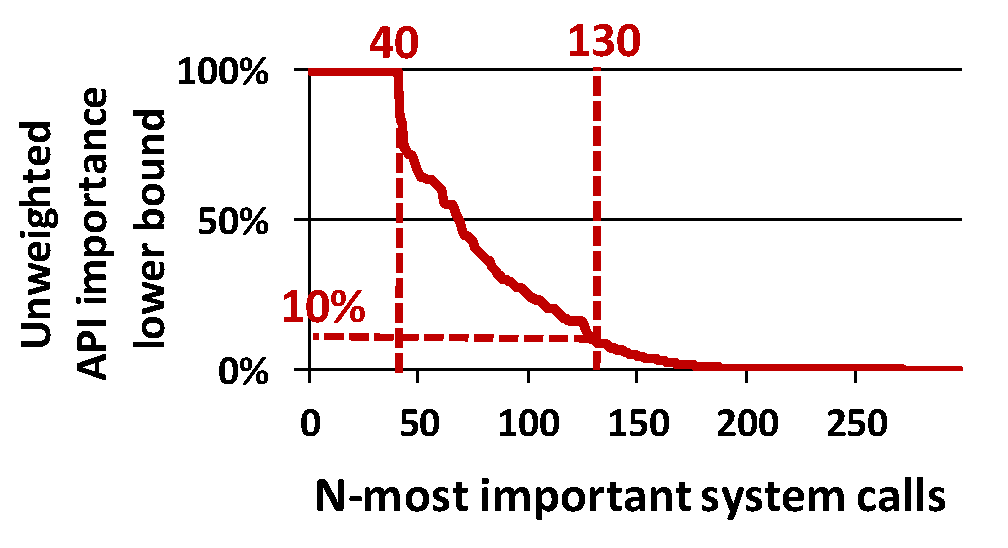
\includegraphics[width=3.6in]{syspop/figures/unweighted-syscall-popularity-all.pdf}
%}
%\footnotesize
%\caption[\Unwusagemetric{} of Linux system calls]
%{The trend of \unwusagemetric{} in N-most important system calls among total \syscallnum{} system calls of \osversion{} with Linux kernel \kernelversion{}.}
%\label{fig:unweighted-syscall-popularity-trend}
%\end{figure}

%We begin by looking at the \unwusagemetric{} of each system call. Figure~\ref{fig:unweighted-syscall-popularity-trend} shows the 
%distribution of system calls across packages. 
%Recall that using \usagemetric{},
%over two-thirds of system calls on Linux are required by 
%at least one application on every installation.
%Using \unwusagemetric{},
%Figure~\ref{fig:unweighted-syscall-popularity-trend} suggests that only 40 system calls are used by all packages,
%and 130 system calls
%are used by at least 10\% of packages.
%%In terms of a prototype maximizing its coverage of potential applications with no concern for overall usability, 130 system calls is the optimal 
%%balance of effort and reward.
%Over half of Linux system calls are used by less than 10\% of packages.  

%%% Thus, changing the security guarantees for just 130 system calls can ensure that 90\% of the packages
%%% are secured. However, we should keep in mind that this does not mean 90\% of the systems are secured as there may be some API used by 
%%% an ubiquitous package that is not secured.

One family of APIs prone to security problems are the %with security issues   that have been considered problematic
{\tt set*id} API family.
%The fundamental problem is that
Many of the {\tt set*id} APIs
have subtle semantic differences across different Unix variants.
%~\citep{chen02setuid}.
Chen et al.~\citep{chen02setuid} conclude that 
{\tt setresuid} has the clearest semantics 
across all Unix flavors. 
%BSD, System V and Linux have different interpretation of 
%other uid-setting system calls such as setuid, setreuid and seteuid. 
Table~\ref{tab:syspop:secure-api} shows the \unwusagemetric{} 
of {\tt set*id} and {\tt get*id} system calls.
Most packages have 
adopted the more clear and secure interface. 
System calls {\tt setuid}, {\tt setreuid}, and {\tt setresuid} have
\unwusagemetric{} of 15.67\%, 1.88\% and 99.68\% respectively. 
%However, some packages
%are still using the older interfaces, and package maintainers or distribution security teams
%may want to push patches to these lingering instances more aggressively.
%The \unwusagemetric{} trend of {\tt set*gid} is similar to
%that of {\tt set*uid}.
However, for {\tt get*id} system calls, the \unwusagemetric{} suggests that the {\tt getres*id}
system calls %with the clearest semantics are not preferred.
are only used by roughly 36\% of packages.
%Package maintainers or distribution security teams
%may want to rectify this case.

Directory operations have a long history of exploitable race conditions~\citep{tocttou-truck, wei05fast, races-usenix05}, or time-of-check-to-time-of-use (TOCTTOU) vulnerabilities.
%Another security concern that exists in file system calls that operate on dire
%is {\em atomicity}.
In a privileged application, one system call (e.g., {\tt access}) checks 
the user's permission, and a second call operates on the file.
%This system call is primarily used
%by privileged applications, such as setuid-to-root binaries.
%The {\tt access} call is used to avoid potential ``confused deputy'' problems~\citep{Hardy:1988:CD:54289.871709},
%by determining the invoking user's authority
%by checking the access rights of the calling process's real UID and GID
%instead of the effective ID.
%The problem is that {\tt access}
%are vulnerable to 
%time-of-check-to-time-of-use (TOCTTOU) attacks~\citep{tocttou-truck}.
%The attacker can change the resource's state 
%between the check and the use in such a way that it invalidates the results of the check.
There are countermeasures that effectively walk the directory
hierarchy in user space~\citep{tsafrir08tr}.
This approach replaces calls like {\tt access} with {\tt faccessat},
and similar variants.
%The atomic version of these system calls, such as
%{\tt faccessat}, avoids this attack by interpreting the path relative to
%an already open file descriptor~\citep{tsafrir08tr}.
Table~\ref{tab:syspop:secure-api} shows the current \unwusagemetric{} of
{\tt *at} system call variants and their older counterparts.
We observed that the \unwusagemetric{} of
the race-prone {\tt access} is still high (74.24\%), whereas {\tt faccessat} is only 0.63\%.
This suggests about 75\% of the
packages use the more vulnerable {\tt access} system call instead of the more secure one.
%This indicates that perhaps more outreach is needed on this issue.
%Similar to {\tt access} and {\tt faccessat}, a few more system calls designed to prevent TOCTTOU attacks
%are shown in
%more of this types of system call variants.
%The \unwusagemetric{} trend for the other system calls is similar, except for
%{\tt fstat} and {\tt newfstatat} which are both ubiquitously used.

\begin{table}[t!b!]
\footnotesize
\centering
\begin{tabular}{m{1.2in}>{\raggedleft\arraybackslash}m{1.2in}m{1.2in}>{\raggedleft\arraybackslash}m{1.2in}}
\toprule
{\bf Insecure API} & {\bf \UnwusageMetric{}} & {\bf Secure API} & {\bf \Unwusagemetric{}}\\
\midrule
\multicolumn{4}{c}{\bf Unclear vs. Well-defined ID Management Semantics} \\
\midrule
\addlinespace
{\tt setuid}   & 15.67\% & \multirow{2}{*}{\tt setresuid} & \multirow{2}{*}{99.68\%} \\
{\tt setreuid} &  1.88\% & & \\
\addlinespace {\tt setgid}   & 12.07\% & \multirow{2}{*}{\tt setresgid} & \multirow{2}{*}{99.68\%} \\
{\tt setregid} &  1.24\% & & \\
\addlinespace
{\tt getuid}   & 99.81\% & \multirow{2}{*}{\tt getresuid} & \multirow{2}{*}{36.19\%} \\
{\tt geteuid}  & 55.15\% & & \\
\addlinespace
{\tt getgid}   & 99.81\% & \multirow{2}{*}{\tt getresgid} & \multirow{2}{*}{36.14\%} \\
{\tt getegid}  & 48.87\% & & \\
\addlinespace
\midrule
\multicolumn{4}{c}{\bf Nonatomic vs. Atomic Directory operations} \\
\midrule
{\tt access}   & 74.24\% & {\tt faccessat}  & 0.63\% \\
\addlinespace
{\tt mkdir}    & 52.07\% & {\tt mkdirat}    & 0.34\% \\
%\addlinespace
%& {\tt mknod}    &  5.86\% & {\tt mknodat}    & 0.26\% \\
%\addlinespace
{\tt rename}   & 43.18\% & {\tt renameat}   & 0.30\% \\
%\addlinespace
%& {\tt symlink}  & 21.93\% & {\tt symlinkat}  & 0.34\% \\
%\addlinespace
{\tt readlink} & 46.38\% & {\tt readlinkat} & 0.50\% \\
\addlinespace
%& {\tt link}     & 28.04\% & {\tt linkat}     & 0.28\% \\
%\addlinespace
%& {\tt utimes}   & 17.90\% & {\tt futimesat}  & 0.20\% \\
%\addlinespace
%& {\tt chown}    & 24.59\% & \multirow{2}{*}{\tt fchownat}   & \multirow{2}{*}{ 0.23\%} \\
%& {\tt fchown}   & 27.14\% & & \\
{\tt chown}    & 24.59\% & {\tt fchownat}   & 0.23\% \\
{\tt chmod}    & 39.80\% & {\tt fchmodat}   & 0.13\% \\
%& {\tt stat}     & 99.80\% & \multirow{2}{*}{\tt newfstatat} & \multirow{2}{*}{99.79\%} \\
%& {\tt fstat}    & 99.80\% & & \\ {\tt stat}     & 99.80\% & {\tt newfstatat}   & 99.79\% \\
%& {\tt chmod}    & 39.80\% & \multirow{2}{*}{\tt fchmodat}   & \multirow{2}{*}{ 0.13\%} \\
%& {\tt fchmod}   & 32.78\% & & \\
\bottomrule
\end{tabular}
\caption[\Unwusagemetric{} of secure and insecure API variations]
{\Unwusagemetric{} of secure and insecure API variations. Higher is more important.}
\label{tab:syspop:secure-api}
\end{table}


In addition to security-related hints, \unwusagemetric{}
indicates whether obsolete APIs have been replaced by newer variants.
%\fixmedp{Skimming the waitit manual, it is not obvious that wait4 is actually obsolete;
%in fact, I think it is system-specific and more precise (similar to dup3 below).}
For instance, {\tt wait4} system call is considered obsolete~\citep{wait4man},
and the alternative {\tt waitid} is preferred, as it more precisely specifies which child state changes to wait for. %\fixmetsai{kernel version? cite?}\fixmedp{why?}
However, \unwusagemetric{} of {\tt wait4} and {\tt waitid} is 60.56\% and 0.24\%, respectively.
This indicates that 60\% of the packages are still using the older {\tt wait4} system call.
%This is another area of concern that needs to be notified to the maintainers of these packages.
Table~\ref{tab:syspop:new-api} shows similar trend for some other system calls.
Our dataset provides more opportunity for system developers
to actively communicate with application developers,
in order to speed up the process of retiring problematic APIs. 

%\callout{Adoption of newer, preferred API variants is often slow, and 
%kernel developers could benefit from an easy mechanism to identify
%relevant developers.}

Some APIs are specific to a particular OS,
such as Linux,
and often have more portable variants.
Table~\ref{tab:syspop:linux-specific} shows the comparison between
Linux-specific APIs and their generic variants.
The results show most developers prefer portable or generic APIs
more than Linux-specific APIs.
Except {\tt pipe2}, most API variants that are Linux-specific
have \unwusagemetric{} lower than 10 percent.
\fixmedp{Can you comment on why pipe2 is popular?}
%Moreover, \unwusagemetric{} also gives us insights about developer preference over multiple versions of similar API. For example, whenever possible,
%developers choose the API to maximize the portability of the application. As a result, the \unwusagemetric{} of Linux specific version of system call API is very low compared to their generic counterparts as shown in table ~\ref{tab:linux-specific}.

Finally, we consider system calls with multiple variants
where one version has increased functionality.
%neither is any of them more secure than their siblings.
%Some of them are just alternative to each other,
%or one is simply a more powerful version (more functionality;
%accepting more arguments) of the other.
%The existence of these API variants is caused by arbitrary choices
%made by the OS developers.
%In addition to some system call variants being Linux specific, in some cases, that is not the factor for developer preference of one API variant over the other.
Table~\ref{tab:syspop:prefer-api} shows the difference %of \unwusagemetric{}
between these system calls.
%which are either alternative to each other,
%or one is simply a more powerful version (more functionality; accepting more arguments) of the other.
%In a few cases, like {\tt recvfrom} or {\tt sendto},
%a significant fraction of the developers choose
%the more powerful version of the system calls ({\tt recvmsg} or {\tt sendmsg})
%or more functionality. 
Interestingly, more developers chose the less powerful variants,
such as using {\tt select} over {\tt pselect6}, or {\tt dup2} over {\tt dup3}.
This indicates that more often than not, developers choose simplicity 
unless a task demands the functionality of a more powerful API variant.

\begin{table}[bhp!]
\footnotesize
\centering
\begin{tabular}{m{.2\linewidth}>{\raggedleft\arraybackslash}m{.2\linewidth}m{.2\linewidth}>{\raggedleft\arraybackslash}m{.2\linewidth}}
\toprule
{\bf Old API} & {\bf \UnwusageMetric{}} & {\bf New API} & {\bf \UnwusageMetric{}}\\
\midrule
{\tt getdents} & 99.80\% & {\tt getdents64} & 0.08\% \\
\addlinespace
{\tt utime} & 8.57\% & {\tt utimes} & 17.90\% \\
\addlinespace
{\tt fork} & 0.07\% & \multirow{2}{*}{\tt clone} & \multirow{2}{*}{99.86\%} \\ 
{\tt vfork} & 99.68\% & & \\
\addlinespace
{\tt tkill} & 0.51\% & {\tt tgkill} & 99.80\% \\
\addlinespace
{\tt wait4} & 60.56\% & {\tt waitid} & 0.24\% \\
\bottomrule
\end{tabular}%
\caption[\Unwusagemetric{} of old and new API variations.]
{\Unwusagemetric{} of old (generally deprecated) and new (preferred) API variations. Higher is more important.}
\label{tab:syspop:new-api}
\end{table}%


\begin{table}[bhp!]
\footnotesize
\centering
\begin{tabular}{m{.2\linewidth}>{\raggedleft\arraybackslash}m{.2\linewidth}m{.2\linewidth}>{\raggedleft\arraybackslash}m{.2\linewidth}}
\toprule
{\bf Linux Specific API} & {\bf \Unwusagemetric{}} & {\bf Portable / Generic API} & {\bf \Unwusagemetric{}}\\
\midrule
{\tt preadv} & 0.15\% & {\tt readv} & 62.23\% \\
%\addlinespace
{\tt pwritev} & 0.16\% & {\tt writev} & 99.80\% \\
\addlinespace
{\tt accept4} & 0.93\% & {\tt accept} & 29.35\% \\
\addlinespace
{\tt ppoll} & 3.90\% & {\tt poll} & 71.07\% \\
\addlinespace
{\tt recvmmsg} & 0.11\% & {\tt recvmsg} & 68.82\% \\
%\addlinespace
{\tt sendmmsg} & 5.17\% & {\tt sendmsg} & 42.49\% \\
\addlinespace
{\tt pipe2} & 40.33\% & {\tt pipe} & 50.33\% \\
\bottomrule
\end{tabular}%
\caption[\Unwusagemetric{} of other API variants]
{\Unwusagemetric{} of other API variants,
and comparison between Linux-specific versions and more portable or generic versions. Higher is more important.}
\label{tab:syspop:linux-specific}%
\end{table}%


\begin{table}[bhp!]
\footnotesize
\centering
\begin{tabular}{m{.2\linewidth}>{\raggedleft\arraybackslash}m{.2\linewidth}m{.2\linewidth}>{\raggedleft\arraybackslash}m{.2\linewidth}}
\toprule
{\bf Linux API} & {\bf \Unwusagemetric{}} & {\bf Alternative API} & {\bf \Unwusagemetric{}}\\
\midrule
{\tt read} & 99.88\% & {\tt pread64} & 27.23\% \\
{\tt select} & 61.53\% & {\tt pselect6} & 4.13\% \\
\addlinespace
\multirow{2}{*}{\tt dup3} & \multirow{2}{*}{8.72\%} & {\tt dup2} & 99.75\% \\
& & {\tt dup} & 66.64\% \\
\addlinespace
{\tt recvmsg} & 68.82\% & {\tt recvfrom} & 53.80\% \\
{\tt sendmsg} & 42.49\% & {\tt sendto} & 71.71\% \\
%\addlinespace
%{\tt chdir} & 44.61\% & {\tt fchdir} & 2.20\% \\
\bottomrule
\end{tabular}%
\caption[\Unwusagemetric{} among similar API variants]
{\Unwusagemetric{} among similar API variants. Higher is more important.}
\label{tab:syspop:prefer-api}%
\end{table}%

 
%\callout{Developers  prefer the most portable or the simplest API option among variations of same system call.}

\section{Implications for System Developers}
\label{sec:syspop:analysis}

The statistics in Section~\ref{sec:observation} can inform decisions of application developers, library developers,
and kernel developers.  Similarly, the ability to easily generate a comprehensive data set of API footprints
has several practical uses.

% to make well informed decisions that may affect the efficiency, security and compatibility of the system.

%As a side-effect of our study, we generate a system call profile for every 
%application binary i.e., we determine what are the possible system calls 
%made by a given application either directly to the kernel or via a 
%dynamically linked library. 

One practical benefit of this study is the ability to automatically identify a system call profile of
every application distributed with \osdist{}. In fact, we observed that the total 31,433 applications 
have 11,680 different system call footprint and 9,133 out of these applications have a unique system call footprint.
We note that these numbers may vary with dynamic analyses, but the fact that one third of all Debian/Ubuntu applications
have a unique system call footprint is interesting.

System call footprints have been explored previously for identifying malware or software compromises~\citep{policy-extraction}. %\fixmedp{Is this a correct interpretation?}
%This approach has been explored previously in the literature
Linux has recently added seccomp, a Berkeley Packet Filter-based system call filtering framework~\citep{seccomp};
generation of seccomp policies can be easily automated using our framework,
reducing the system's attack surface in the event of an application compromise.

%\callout{We can automatically create system call filters for applications to reduce security risks.}

%%% this has been ond 
%%% Kernel rootkits enter the system by exploiting some vulnerability in the
%%% application and elevating the privilege to modify the system behavior.
%%% The set of system calls or kernel interfaces 
%%% used by an application constitute the bare minimum kernel attack surface 
%%% that needs to be exposed to vulnerabilities in that particular application.
%%% However, unless the access of kernel interface is limited to only this minimal set,
%%% all the linux interfaces are exposed to the vulnerabilities in the application.
%%% Linux kernel v3.5 added the BPF based seccomp support for system call filtering to limit which
%%% syscalls can be called by a process/application. 
%%% As a side-effect of our study, we generate a system call profile for every 
%%% application binary i.e., we determine what are the possible system calls 
%%% made by a given application either directly to the kernel or via a 
%%% dynamically linked library.
%%% We can easily automate the conversion of this system call profile generated
%%% by our analysis for each application to seccomp filter rules.
%%% These seccomp rules can reduce the attack surface available to vulnerability exploits in the application,
%%% improving the overall security of the system.

%\fixmedp{From here down is a little repetitive.  It is ok, but I think this has been covered elsewhere, or could be merged up into the appropriate section}
These tools can also help OS developers evaluate when it is safe to remove a deprecated interface,
or when interfaces appear to be irrelevant to most users (e.g., {\tt remap\_file\_ pages}).
In the case of an irrelevant interface, this may either indicate something is a candidate for deprecation (e.g., {\tt lookup\_dcookie}),
or that a useful or important feature (e.g., {\tt faccessat}) is not getting sufficient traction.
Linux developers currently wait as long as 
six years to retire an interface, allowing ample time for application and library developers to change.
% let the applications and libraries to change the use of deprecated ABI before it is completely dropped. 
Our dataset and methodology can allow more proactive outreach and more rapid system evolution.
%The reason for this long wait is that the kernel developers have no way of knowing if there is any application in the wild
%still using the interface to be deprecated. Using our system, the kernel developers can be proactive and
%notify the maintainers of only those applications that are affected by the change. 

%%% Apart from helping new OS developers to maintain compliance to Linux ABI based on the metric discussed in section \S\ref{sec:measure},
%%% our popularity distribution can also help kernel developers to choose the interfaces to be deprecated.
%%% More the number of interfaces to kernel, bigger is the available attack surface. Thus, it is desirable to
%%% remove some of the less popular interfaces to reduce the attack surface. Moreover, maintaining each
%interface incurs additional effort for kernel developers. 

%% dp:  meh
%%% Apart from just removing the
%%% interfaces no longer used by any application, the kernel developers can also move the less popular system calls
%%% to optional ioctl calls provided by dynamically loaded kernel modules. In fact, the kernel developers can
%%% just notify particular libraries to handle the missing syscall by registering for seccomp upcall so that
%%% the libraies can load the required kernel module at runtime if needed.
%%% Moreover, this syscall popularity
%%% distribution can provide the application and library developers a good approximation of the possible candidates for
%%% deprecation so that they can avoid refactoring the code by avoiding use of least popular interfaces especially 
%%% if there is another popular alternative is available.

The \libc{} function call popularity can similarly help library developers to remove function calls that
are not used (222 functions). 
Moreover, the function call importance distribution can also help reduce the library's memory footprint by
organizing the in-memory layout by importance.
%Unimportant functions will never be demand-paged in on many systems.
% 2MB is a little underwhelming
%%% Although \libc{}'s text segment is only about 2MB, this could be a non-trivial improvement for 
%%% embedded devices, and potentially reduce the need for 
%%% loading the code for only most popular functions in memory. While the reduction in memory footprint is small
%%% it is still substantial for embedded devices. For instance, the total \libc{} text section is only about 2MB.

% dp: I also think this is  a reach
\begin{comment}
The x86 processor fetches instructions at the order of cacheline size and usually have an prefetch hardware
that learns sequential or step-based access patterns of memory and prefetch those instructions or data before
it is actually needed. The performance of an application can be highly optimized if there are very low number of
cache misses and if the prefetch hardware can always fetch the right data or instruction.
The compilers know about the details of target architecture and can organize the code to optimize the code
for the target architecture. Using the \libc{} function call popularity, the compilers can place the most frequently used code
together causing less cacheline misses. The least popular part of the library will be demand loaded in memory only if it is accessed.
In fact, this approach can help reduce the working memory set of the application without even any need for special case handling.
For instance, 46\% of all the function call constitute the top 90\% of the most popular function calls. 
\end{comment}

%Commands to get the numbers for this calculation.
% grep -n -e '0\.09' libc-popularity.csv | head -n 1 | cut -d ":" -f 1
% wc -l libc-popularity.csv



%Popularity of system calls can help kernel developers decide on which system calls can be easily deprecated.


%1. Which syscalls/function calls to deprecate?
%	- Help application developers to choose popular system calls as they have lower risk of being deprecated. Application developers do not have to refactor the code if they can avoid the
%	  potential candidates for deprecation.

%2. Help compiler tools to load only most popular system calls in memory during linking so that the memory footprint will be reduced and caching can be used much more efficiently
%	- Kernel compilers can also organize the code such that all the code for popular system calls is placed together so that it will cause least number of cache line misses and be easy to prefetch.

%3. Automatically generate sandbox profiles and reduce the attack surface of OS/library/application

%4. Case study the most used and unused syscalls and find the reason behind them.
%	If the answer is because \libc{} decided to do so, find out if a syscall is used by \libc{} but not by any application, we need to figure out why?

%5. Make popular vector calls/fs access as syscalls and make less popular ones as optional ioctls.

%%=======Inferences=======
%1. syncfs is less prefered over sync by developers.
%2. security which is undefined is used by librsbac.so.1.0.0 but everyone now uses librsbac.so.1 instead which doesnt use security
%3. numa based syscalls have very low popularity - get\_mempolicy, set\_mempolicy, numactl, sched\_getaffinity, sched\_setaffinity, move\_pages, migrate\_pages.
%4. Recently added syscalls like finit_module, kcmp have lower popularity.
%5. Pople use setresuid and getresuid more often than confusing and distribution dependent setuid/setreuid thanks to setuid demystified paper.




% Unused System Calls & Possible reason for not using
% get\_kernel\_syms & Removed in 2.6
% getpmsg, putpmsg, tuxcall & Unimplemented
% io\_getevents, restart\_syscall, rt\_tgsigqueueinfo, kcmp, finit\_module & No \libc{} wrapper for this system call
% lookup\_dcookie & special-purpose system call only used by oprofile profiler
% epoll\_ctl\_old, epoll\_wait\_old & Replaced by epoll\_ctl and epoll\_wait
% semtimedop & Timeout option for semop which is by itself not popular(0.162)
% migrate\_pages, move\_pages & Applicaitons are not NUMA-aware
% recvmmsg, sendmmsg & Linux specific. Other generic syscalls like recvmsg(0.968) and sendmsg(0.808) are prefered.
% clock\_adjtime & Added in 2.6.39 to support Precision Time Protocol. Other system call adjtimex(0.021) is prefered
% process\_vm\_readv, process\_vm\_writev & Nonstandard Linux extensions. No atomicity guarantee.




%%%% Unused system calls %%%%

% get_kernel_syms Removed in 2.6
% getpmsg The getpmsg() function shall be equivalent to getmsg(), except that it provides finer control over the priority of the messages received. - Unimplemented
% putpmsg The putpmsg() function is equivalent to putmsg(), except that the process can send messages in different priority bands. - Unimplemented
% tuxcall Unimplemented
% lookup_dcookie added in 2.6 - return a directory entry's path <=====
% epoll_ctl_old - old
% epoll_wait_old - old
% restart_syscall added in 2.6 - a helper function that restarts a system call <=====
% migrate_pages added in 2.6.16 - move all pages in a process to another set of nodes<===== 
% move_pages added in 2.6.18 - move individual pages of a process to another node <=====
% rt_tgsigqueueinfo added in 2.6.31 - send a signal plus data to a process or thread. These system calls are not intended for direct application use; they are provided to allow the implementation of sigqueue(3) and pthread_sigqueue(3). <=====
% recvmmsg added in 2.6.33  -  receive multiple messages on a socket <=====
% clock_adjtime - add in 2.6.39 - \libc{} doesnt offer the syscall <=====
% sendmmsg added in 3.0 - send multiple messages on a socket <=====


%%%% Least popular syscall (<1%) in ascending order of popularity%%%%

% process_vm_writev - added in 3.2 These system calls are nonstandard Linux extensions. The data transfers performed by process_vm_readv() and process_vm_writev() are not guaranteed to be atomic in any way. These system calls were designed to permit fast message passing by allowing messages to be exchanged with a single copy operation (rather than the double copy that would be required when using, for example, shared memory or pipes). <===== 

% finit_module added in 3.8
% kcmp added in 3.5 - compare  two  processes  to determine if they share a kernel resource
% process_vm_readv - read process_vm_writev details. <=====
% security - Unimplemented system calls  
% getcpu - 2.6.19  determine CPU and NUMA node on which the calling thread is running
% syncfs - 2.6.39 synchronizes just the file system containing file referred to by the open file descriptor fd
% sysfs - 1.2 get file system type information
% get_mempolicy - 2.6.6 retrieve NUMA memory policy for a process
% mq_notify - 2.6.6
% get_thread_area
% set_thread_area
% get_robust_list
% set_mempolicy
% remap_file_pages
% semtimedop
% vserver
% timerfd_gettime
% mbind
% io_getevents
% timer_getoverrun
% uselib
% afs_syscall
% io_destroy
% _sysctl
% query_module
% create_module
% kexec_load
% fanotify_init
% fanotify_mark
% timerfd_settime
% name_to_handle_at
% open_by_handle_at
% timerfd_create
% modify_ldt
% prlimit64
% mq_getsetattr
% tee
% mq_timedsend
% vmsplice
% perf_event_open
% mq_open
% mq_timedreceive
% mq_unlink
% io_cancel
% sched_rr_get_interval
% io_setup
% acct
% io_submit
% rt_sigqueueinfo
% clock_nanosleep
% epoll_pwait
% preadv
% pwritev
% nfsservctl
% ustat
% request_key
% rt_sigpending
% add_key
% getdents64
% timer_gettime
% setfsgid
% setfsuid
% keyctl
% capget
% waitid
% msgrcv
% msgsnd



%%%% Most popular syscall (>90%) in decending order of popularity%%%%

% vfork
% exit_group
% exit
% close
% stat
% fstat
% lseek
% mmap
% munmap
% gettid
% rt_sigprocmask
% write
% open
% read
% writev
% getrlimit
% getuid
% sched_yield
% getcwd
% getdents
% futex
% clock_getres
% getpid
% getgid
% fcntl
% tgkill
% clone
% lstat
% dup2
% newfstatat
% openat
% execve
% kill
% setpgid
% setresuid
% setresgid
% sched_setscheduler
% pread64
% sched_setparam
% ioctl
% madvise
% mprotect
% rt_sigreturn
% rt_sigaction
% set_tid_address
% set_robust_list
% 


\section{Implementation Details}
\label{sec:syspop:framework}

This section provides additional implementation details of our analysis framework. % for mining the API footprint for ELF executables and libraries.

%Analyzing the footprint of an applications requires interpretation of its behavior. As discussed in section~\ref{sec:measure:analysis}, we choose to build our framework by using {\bf static analysis} technique instead of dynamic analysis. The reason is that static analysis can trace potential executions of the applications, regardless of the runtime coverage of the code.

Our analysis is based on disassembling binaries inside each application package, using the standard {\tt objdump} tool.
This approach eliminates the need for source or recompilation, and can handle closed-source binaries.
We implement a simple call-graph analysis to detect system calls reachable from the binary entry point ({\tt e\_entry} in ELF headers). 
%\fixmedp{You do actually parse the elf header for e\_entry, right?}
%In our study, we only count executables during measuring both \usagemetric{} and \compatmetric{}.
We search all binaries, including libraries, for system call instructions ({\tt int 0x80}, {\tt syscall} or {\tt sysenter}) or calling the {\tt syscall} API of \libc{}.
We find that the majority of binaries --- either shared libraries or executables --- do not directly choose system calls, but 
rather use the GNU C library APIs.
Among 66,275 studied binaries, only 7,259 executables and 2,752 shared libraries issue system calls.

% system calls. Therefore, analyzing the libraries that an executable depends on is necessary for retrieving a complete set of API footprint.


%, to predict its runtime behaviors.
%The framework requires no scanning of the source code, or recompiling of the applications with additional debug symbols.
%Consider the size and complexity of Ubuntu repositories,
%static analysis of ELF binaries is certainly easier to automate, and is able to analyze the applications that are close-sourced.

%To trace the footprint of applications, it require {\em Call-Graph Analysis} to rip off potential control flows that can eventually lead to usage of system API.
%Challenges of analyzing call-graph is a known issues for researchers in many area such as security, robustness, etc.

Our call-graph analysis allows us to only select system calls that are actually used by the application, not all the system calls that appear in \libc{}.
Our analysis takes the following steps:
\begin{compactitem}
\item For a target executable or a library, generate a call graph of internal function usage.
\item For each library function that the executable relies on, identify the code in the library that is reachable from each entry point called by the executable.
%trace coverage of code in the binary, and generate the minimal subset of the library's footprint that the function could actually link to.
\item For each library function that calls another library call, recursively trace the call graph and aggregate the results. 
\end{compactitem}


Precisely determining all possible call-graphs from static analysis is challenging.
Unlike other tools built on 
call-graphs, such as control flow integrity (CFI), our framework can tolerate the error caused by over-approximating the analysis results.
For instance, 
programs sometimes make function call based on a function pointer passed as an argument by the caller of the function. 
Because the calling target is dynamic, it is difficult to determine at the  call site.
Rather, we track sites where the function pointers are assigned to a register, such as using the {\tt lea} instruction with an address
relative to the current program counter.
%Instead of precisely tracking calling target at the {\tt call} instruction, 
%A function pointer is mostly assigned by {\tt lea} instruction to generate a relative address to the current program counter. 
This is an over-approximation because, rather than trace the data flow, we assuming that a function pointer assigned to a local variable will be called.
This analysis could be more precise if it included a data flow component. 
%\fixmedp{As an aside, this level of data flow analysis shouldn't be that hard, right?  Not  that it matters, except for the thesis/journal version.}

We also hard-code for a few common and problematic patterns.
For instance, we generally assume that the registers that pass a system call number to a system call,
or an opcode to a vectored system call, are not the result of arithmetic in the same function.
We spot checked this assumption, but did not do the data flow analysis to detect this case.

%must trace the register values such as {\tt RAX/EAX} for system call number or {\tt RBX/EBX} for parameter to vectored system calls. 

%Based on {\em Case-by-case study}, we assume no arithmetic but direct assignment of integers is possible when the program is issuing a system call. 

%If our analysis cannot precisely determine whether an API is used, we 
%err on the side of assuming an API is used.

%In the case of a run

%allow slightly enlarge the traced footprint of application, to gain simplicity for complex call-graph analysis corner cases. 
%For the specific run-time scenario of the application that can hard to interpret, we do a {\bf Case-by-Case study} to find out strategy of analyze the footprint practicably.

%  that call-graph analysis is complex for generating the accurate control flow of the run time. Fortunately, unlike other studies that relies on 

%In our study, we specifically call it {\bf Over-approximation}. 


%The following is a few example of using {\bf Over-approximation} and {\bf Case-by-Case study} to simplify call-graph analysis:
%\begin{compactenum}
%\item 
%\item 
%\end{compactenum}

Finally, the last mile of the analysis is to recursively aggregate footprint data. We insert all raw data into a {\tt Postgresql} database, and 
use recursive SQL queries to generate the results. 
To scan through all \packagenum{} packages in the repository, collect the data, and generate the results takes roughly three days.

   




%\section{Evaluation}
%\label{sec:eval}
%\note{about 1.5page}

\begin{table}[t]
\footnotesize
\centering
\begin{tabular}{p{2.45in} r}
\toprule
\textbf{Evaluation Criteria} & \textbf{Size}\\
\midrule
\addlinespace
Source Lines of Code (Python) & 3,105 \\
\addlinespace
Source Lines of Code (SQL) & 2,423 \\
\addlinespace
Total Rows in Database & 428,634,030 \\
%\addlinespace
%Missed/Unknown system call instances & 1,643\\
%\addlinespace
%Missed/Unknown vectored call instances & 2,212\\
\bottomrule
\end{tabular}%
\caption{Implementation of the API usage analysis framework.}
\label{tab:syspop:eval}%
\end{table}%

Our implementation is summarized in Table~\ref{tab:syspop:eval}.
We wrote 3,105 lines of code in Python and 2,423 lines of code in SQL (Postgresql).
The database contains 48 tables with over 428 Million entries.
%\rev{Update false-negative}
%{Due to the limitations of our approach,
%we cannot identify the system call numbers at 4.2\% of system call locations,
%and the opcodes at 3.7\% of vectored system call locations,
%among all binaries studied.}
%\fixmedp{I still don't understand what this means.  How did you know you missed some?}
%4.2\% of locations in binary 
%1,643 instances of missed/unknown system call instances
%and 2,212 missed/unknown vectored call instances.
% \fixmedp{What does this mean, exactly?  What does it mean to miss an instance?}

\newpage
\section{Summary}
\label{sec:syspop:summary}

%Based on this study, we can draw several conclusions about the nature of Linux APIs.
%First, for any OS installation in our data set, the required API size
%is several times larger than the \syscallnum{} system calls in Linux, once one considers
%{\tt ioctl} opcodes and files under {\tt /proc}.  A solid two-thirds of system calls are indispensable.
%We show that a substantial range of system calls and other APIs are rarely or even never used.
%And the paper plots a rough guide for adding system calls to a Linux emulation layer or research prototype.
%
%We expect that this data set will be of use to researchers and developers for further analysis,
%Our methodology and tools can be easily applied to future releases and other distributions.
%%\note{about 1/4 pages}
%Our data set, tools, and other information are available at \projecturl{}.

Traditionally,
the routine procedure for system engineers or researchers
to make implementation decisions
is mostly based on their anecdotal knowledge,
which may be partially credible, but heavily skewed toward their preferred or familiar workloads.
The consequence of the lack of information
can be unfavorable for developers who are building innovative systems with legacy application support.
With the binary, bug-for-bug compatibility,
the developers fail to methodologically evaluate and reasonable about
the completeness of API implementation
in their system prototypes,
until the implementation is completed.
As produced by this study,
a principled approach for determining the priority of API implementation,
to enable more applications or more users
that can plausible use the system,
will guide the developers to make more rewarding decisions.


